%!TEX root = ../notes.tex
\section{January 24, 2024}
\label{20240124}

\subsection{Introduction}
The course homepage is at \url{https://cs.brown.edu/courses/csci1515/spring-2024/}, where you can find information such as the \href{https://docs.google.com/document/d/1lvXrMACua9Ma3n2nkLeiRmG-fmjDO1530h22EjkvQ-s/edit?usp=sharing}{syllabus}, projects, homeworks, calendar, lectures and more.

The course is offered in-person in \emph{Bio Med 202}, as well as synchronously over Zoom and recorded asynchronously (lectures posted online). Lecture attendance and participation is highly encouraged!

\textbf{EdStem} will be used for course questions, and \textbf{Gradescope} is used for assignments.

\subsubsection{Staff}

Our course staff have all taken or TA-ed the course before and are excited to help you learn!

Peihan has been at Brown for a couple of years and this was the second time she is teaching this course. Before Brown, she was at the University of Illinois Chicago. Before that, she finished her PhD at UC Berkeley in 2019 with a focus in cryptography. Afterwards, she worked in industry for a couple of years (Visa) before deciding to come back to academia. She still collaborates with industry to see what problems need to be solved in practice.

During her PhD, she started off doing more theoretical cryptography but also did internships and found applied cryptography fascinating as well. Now she works in both.

\subsubsection{Course Philosophy and Logistics}

If look up other \emph{applied} cryptography courses online or at other universities, you will find courses that have ``applied'' in their title. However, if you look at their syllabus or content, it's still mostly theoretical crypto. This may (1) deter students from learning about crypto and (2) leave a gap between theoretical crypto and crypto in practice. (2) is bad because if someone makes a mistake in the crypto domain, the consequences are often significant.

As such, it's helpful for students to get hands-on experience with cryptography:
\begin{itemize}
    \item How cryptography has been used in practice and
    \item How cryptography will be used and implemented in the future.
\end{itemize}

The closest similar course is found at Stanford, which covers theoretical crypto in the first half and more applied crypto in the second. But even that course only covers very basic crypto that are very well established. In the past 10 years or so, there are new and exciting topics in crypto that are gradually becoming more and more common which we will also cover in this course.

For this course, it will be \emph{much less} about math and proofs, and much more about how you can use these tools to do something more fun. It will be coding heavy and all projects will be implemented in C++ using crypto libraries. 

If, however, you are interested in the theoretical or mathematical side, you might consider other courses at Brown like CSCI 1510 and MATH 1580.

% For assignments: \emph{Project 0} is a warmup for C++. Projects 1 \& 2 is to develop secure communication or authentication systems using the underlying cryptographic libraries. The later project, 3, 4 \& 5 will be on more advanced topics. The first 2 are more basic that are developed in practice, and the latter ones are more experimental in practice (so this is recent research in applied cryptography). The final project will be a combination of the existing projects or a project entirely new (separate from the earlier projects, but using the same cryptographic primitives).

% Projects 1 through 5 will be accompanied with homework assignments (appropriately numbered 1 through 5) that develop a conceptual understanding of the materials.

% Projects 1 \& 2 are to be done individually, the later projects are done in pairs (you can choose to go solo if you so wish as well). You are encouraged to find partners earlier on to discuss and work with them from the beginning. You are \emph{encouraged} to communicate with your partners on projects 1 \& 2 so you gain a conceptual understanding. You should complete your own write-up and code for the first two projects, however.

There is an option to capstone this course, contact Peihan about this. It would also be best to find a partner who is also capstoning this course.

The following is the grading policy:
\begin{center}
    \begin{tabular}{@{}ll@{}}
        \toprule
        \textit{Type}      & \textit{Percentage} \\ \midrule
        Project 0          & 4\%                 \\
        Projects 1 \& 2    & 20\% (10\% each)    \\
        Projects 3, 4 \& 5 & 36\% (12\% each)    \\
        Homeworks          & 25\% (5\% each)     \\
        Final Project      & 25\%                \\ \bottomrule
    \end{tabular}
\end{center}

You have 4 total late days for \emph{projects}, of which at most two can be used on a single project. Additionally, you have 3 total late days for \emph{homeworks}, of which at most one can be used on a single homework.

All projects are independent, but collaboration is allowed and encouraged. However, you \emph{must write up your own code}.

If you're sick, let Peihan know with a Dean's note.

\subsection{What is cryptography?}

At a high level, \emph{cryptography is a set of techniques that protect sensitive or important information}.

\begin{ques*}
    Where is cryptography used in practice? What guarantees do we want in these scenarios?
\end{ques*}
\begin{itemize}
    \item Online transactions
          \begin{itemize}
              \item When you make a purchase, you might not want people to see your bank balance, what else you have purchased, etc.
              \item You also want to ensure that it was really \emph{you} who purchased the item and not somebody else i.e. authentication
          \end{itemize}
    \item Secure messaging
        \begin{itemize}
            \item End-to-end texting, iMessage
            \item We don't want anyone else to see our messages
        \end{itemize}
    \item Online voting
        \begin{itemize}
            \item Privacy of votes, validity of votes
        \end{itemize}
    \item Databases
        \begin{itemize}
            \item Secure storage
        \end{itemize}
\end{itemize}

\subsection{Secure Communication}
We'll start with the most classic form of cryptography: \emph{secure communication}.

\begin{center}
    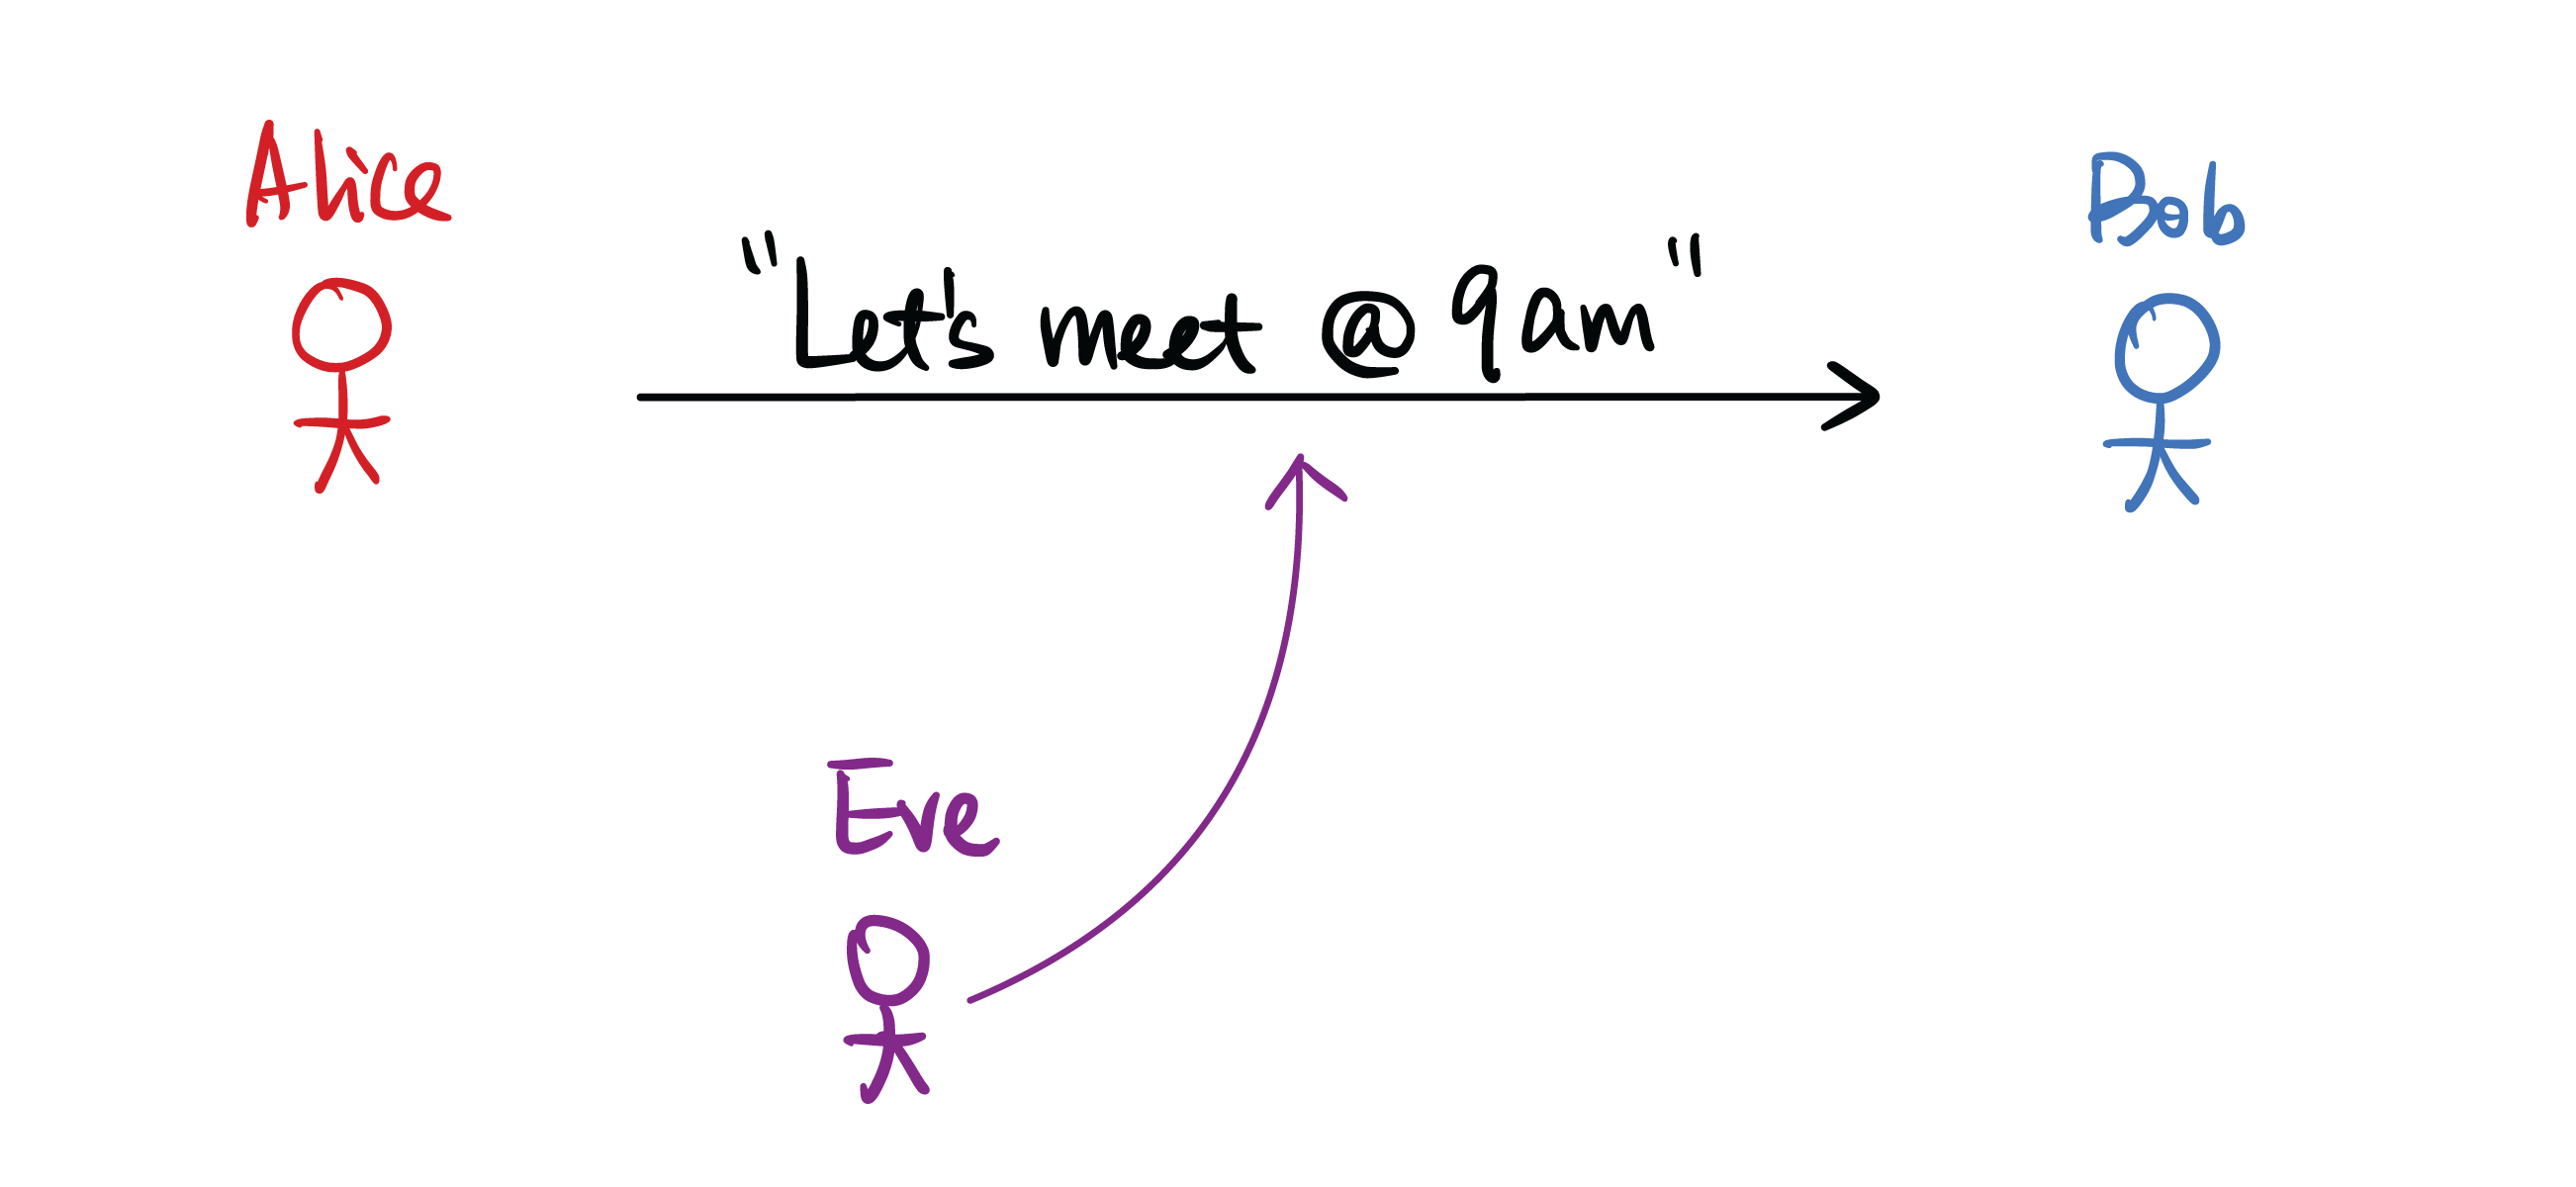
\includegraphics[width=0.8\textwidth]{images/2023-01-26/secure_computation.png}
\end{center}

Assume Alice wants to communicate to Bob ``Let's meet at 9am'', what are some security guarantees we want?

\begin{itemize}
    \item Eve cannot \emph{see} the message from Alice to Bob.
    \item Eve cannot \emph{alter} the message from Alice to Bob. 
\end{itemize}

These two guarantees are the most important guarantees! The former is called \ul{message secrecy}, the latter is called \ul{message integrity}.

\subsubsection{Message Secrecy}

\begin{definition}[Message Secrecy]
    We want cryptography to allow Alice to \emph{encrypt} the message $m$ (which we call \emph{plaintext}) by running an algorithm that produces a \emph{ciphertext} $c$. We call this an \emph{encryption scheme}.

    Bob will be able to receive the ciphertext $c$ and run a \emph{decrypt} algorithm to produce the message $m$ again. This is akin to a secure box that Alice locks up, and Bob unlocks, while Eve does not know the message. The easiest way is for Alice and Bob to agree on a shared secret key.

    \begin{center}
        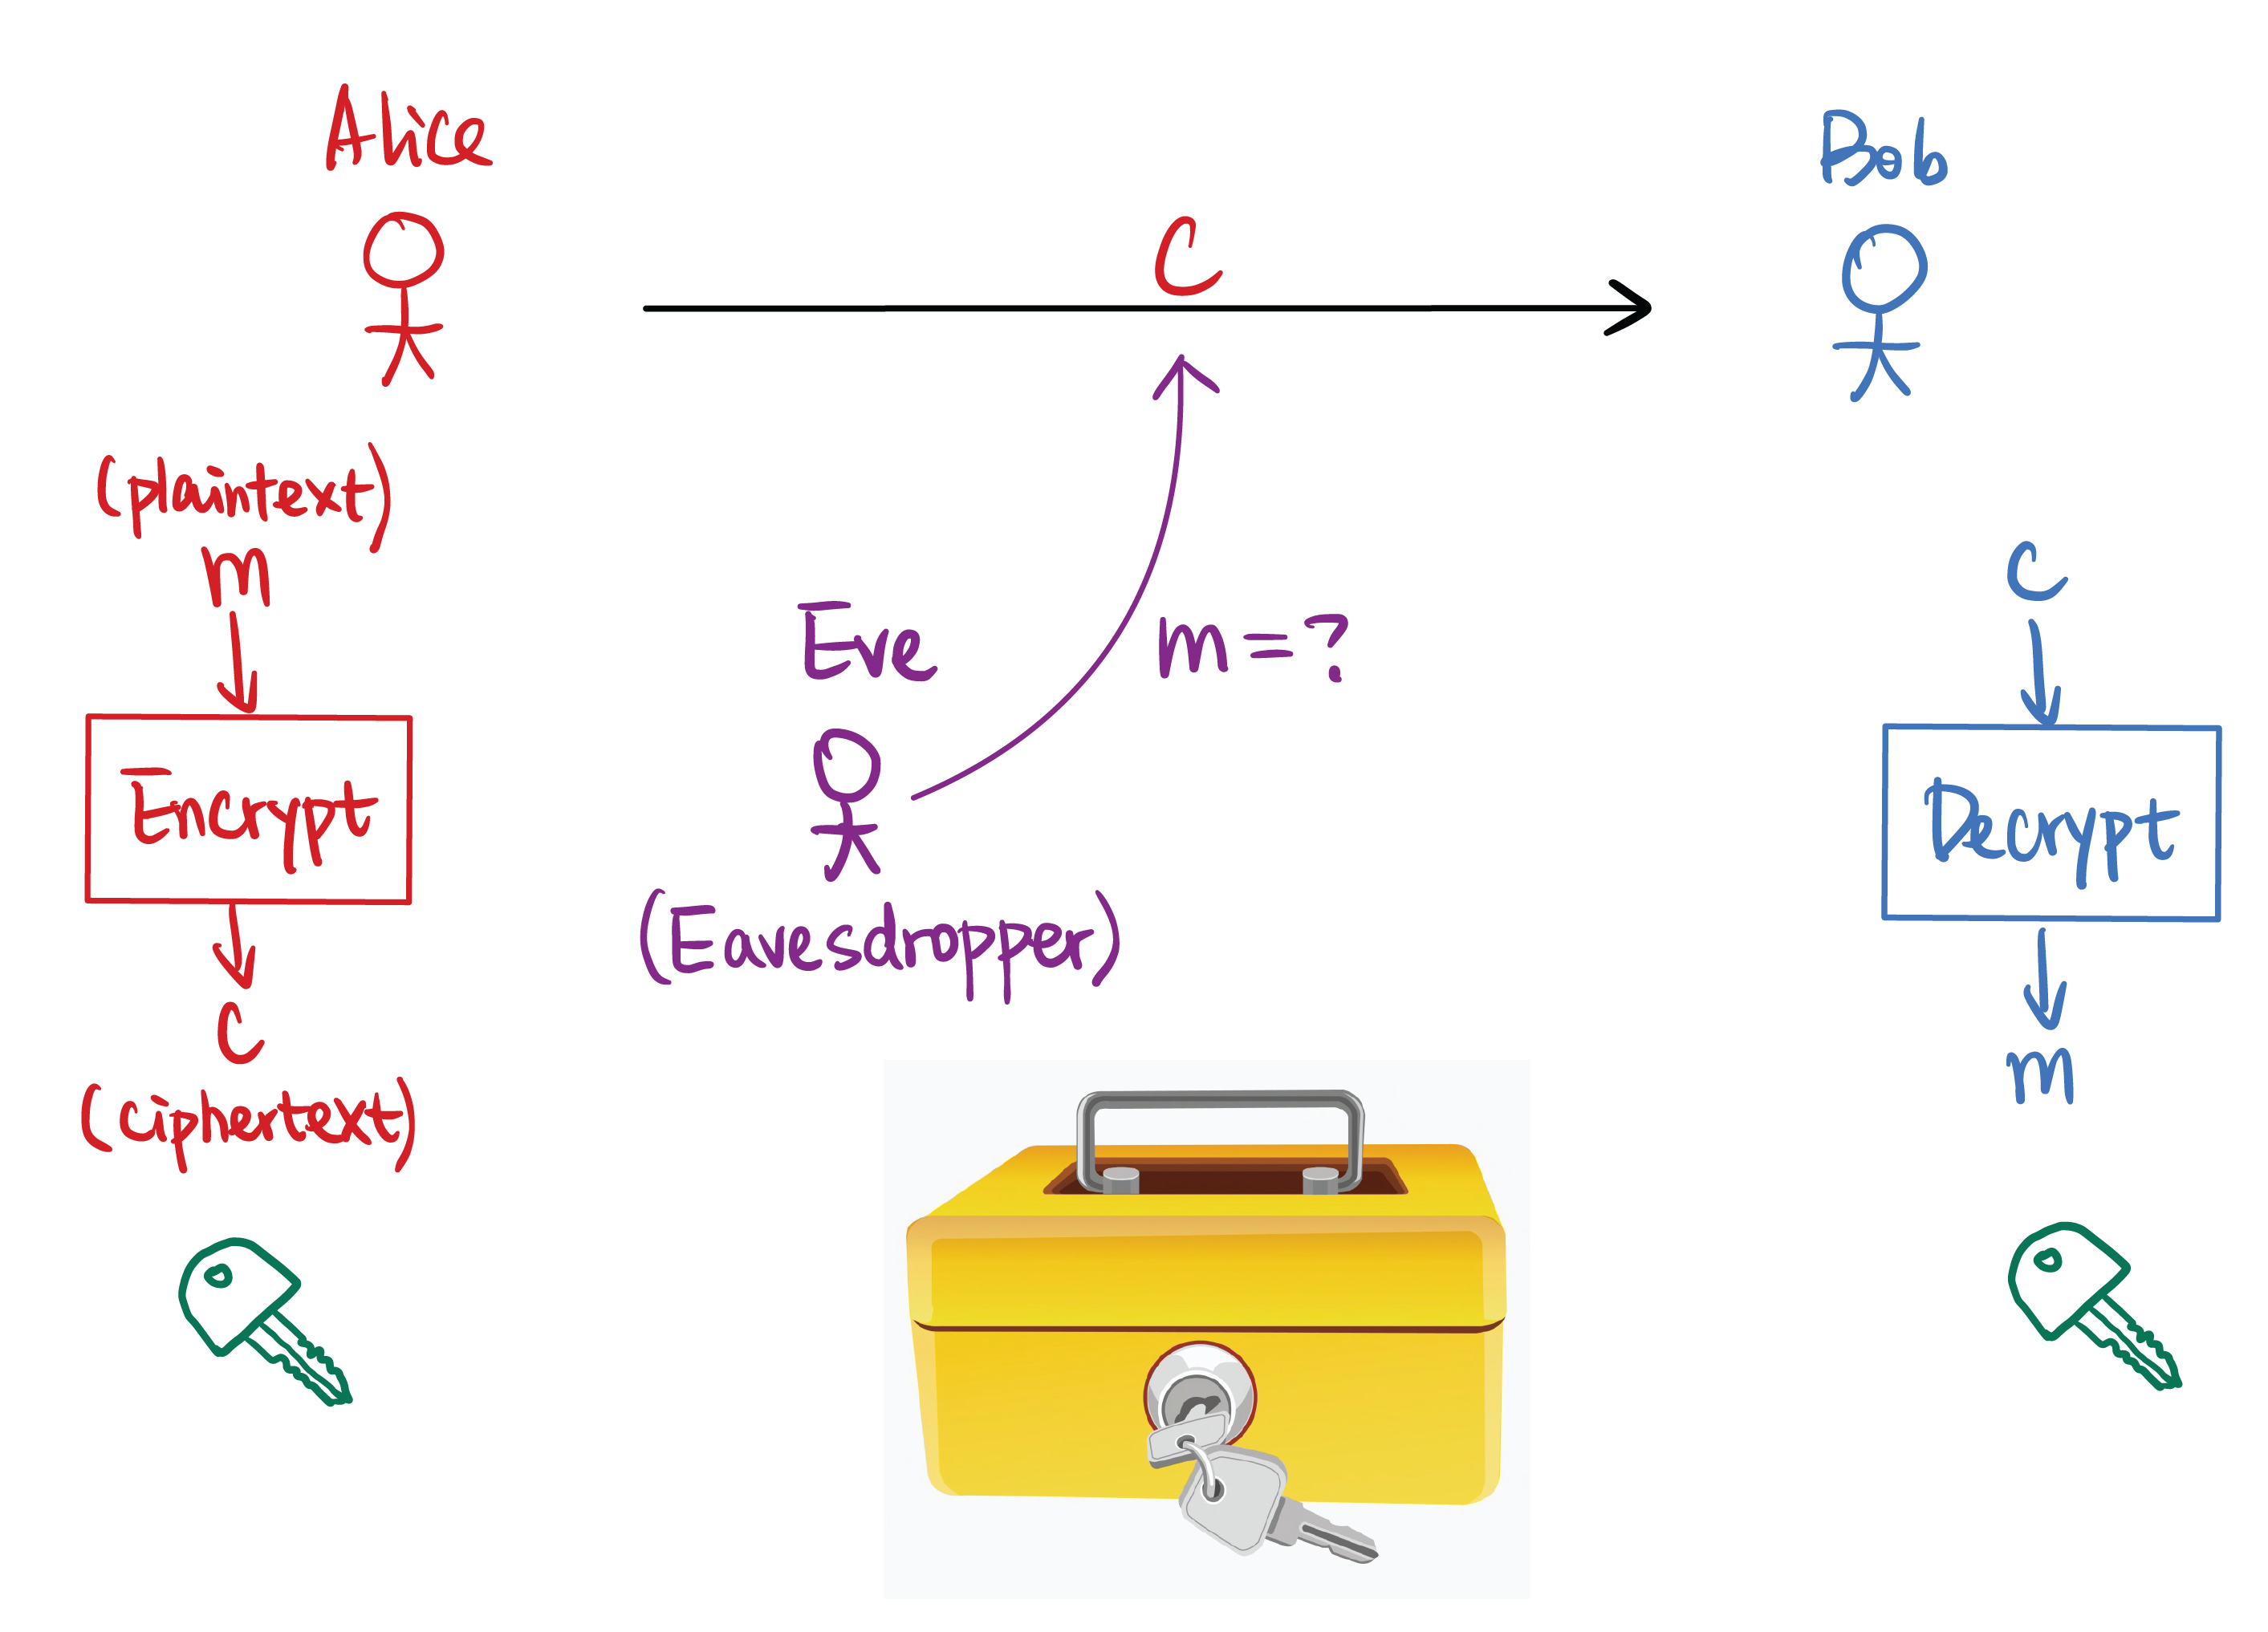
\includegraphics[width=0.8\textwidth]{images/2023-01-26/message_secrecy.png}
    \end{center}

    In this model, Eve is a weaker adversary, an \emph{eavesdropper}. Eve can only see the message, not alter it.
\end{definition}

\begin{example}[Substitution Cipher]
    The key that Alice and Bob jointly uses is a permutation mapping from $\{A\dots Z\}\to \{A\dots Z\}$. This mapping is the \emph{secret key}.

    Bob also has the mapping, and takes the inverse of the permutation to retrieve the message.

    \begin{center}
        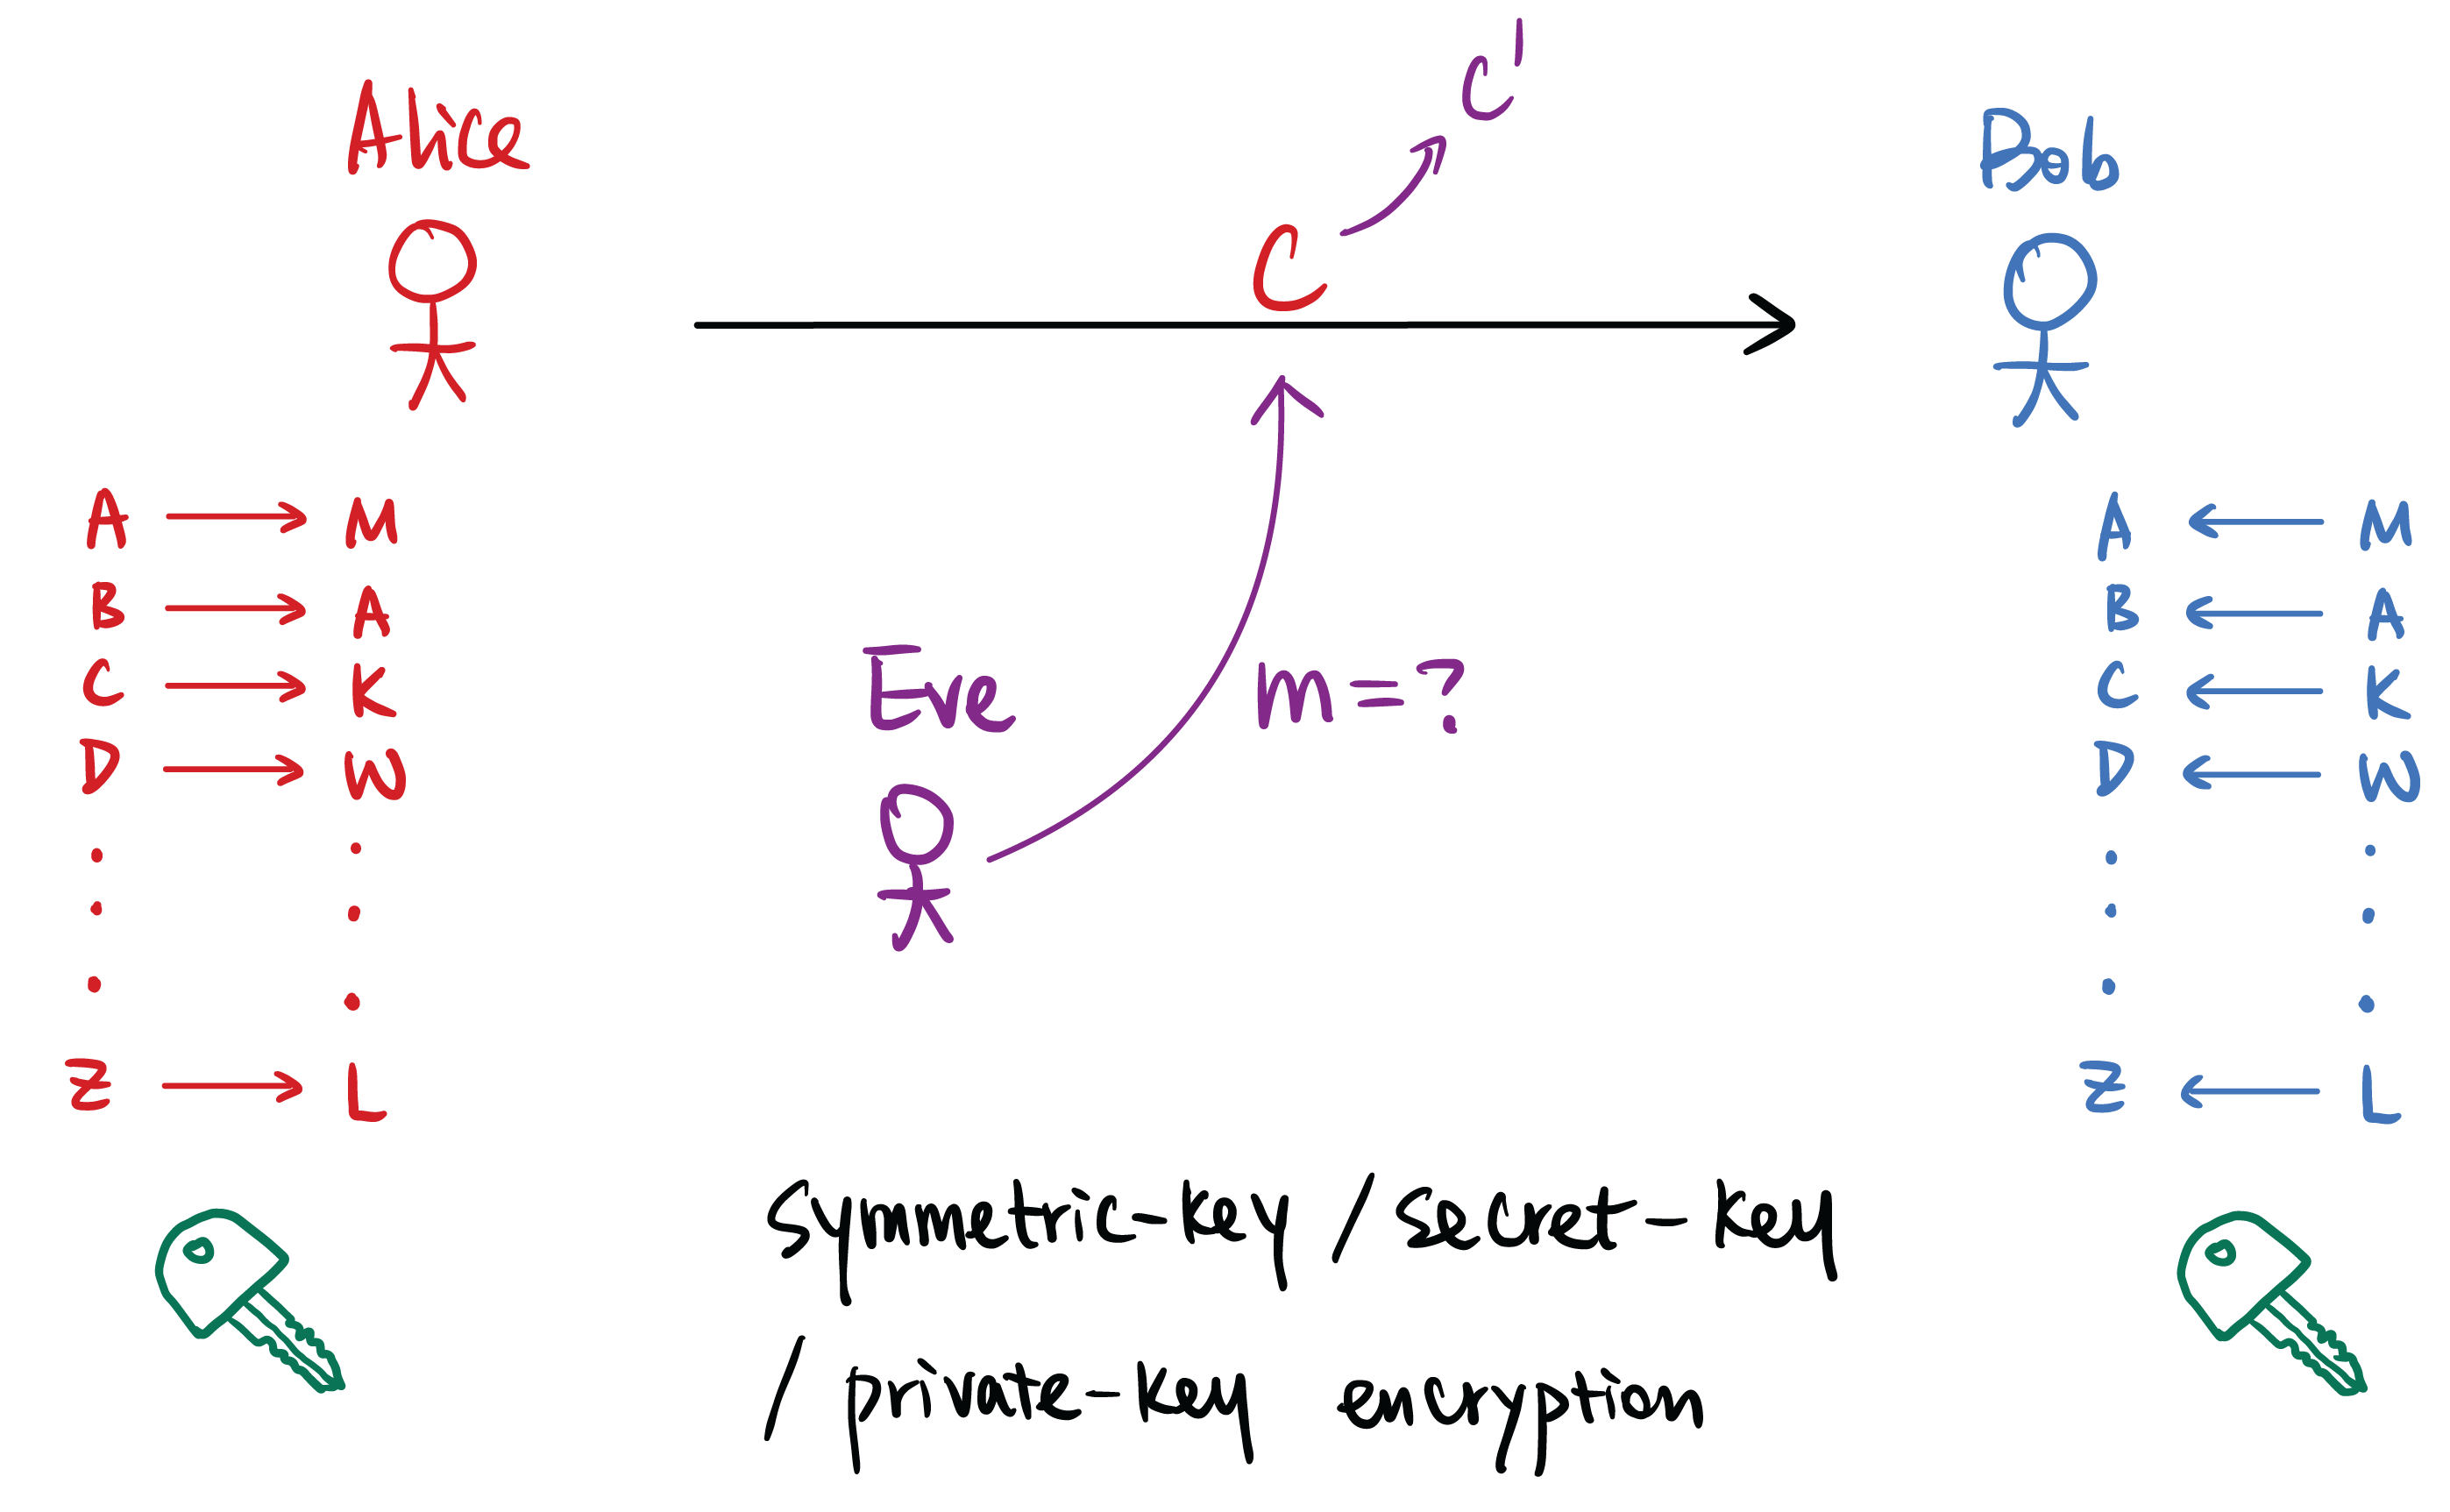
\includegraphics[width=0.9\textwidth]{images/2023-01-26/substitution_cipher.png}
    \end{center}

    This scheme is not quite secure! \emph{Why?}

    Given a large enough text, you can apply frequency analysis and break the substitution cipher.
\end{example}
\begin{remark*}
    This encryption scheme also requires that Alice and Bob meet up in person to exchange this shared private key. Schemes like this are called \emph{symmetric-key, secret-key, or private-key encryption}. They need to somehow agree first on the same secret key.
\end{remark*}

\begin{definition}[Public-key Encryption]
    There is another primitive that is much stronger: \ul{public-key encryption}. Bob publishes both a \emph{public} key and a \emph{private} key. You can consider a lock where you don't need a key to lock it\framedfootnote{You literally click it closed}, and only Bob has the key to unlock it.

    \begin{center}
        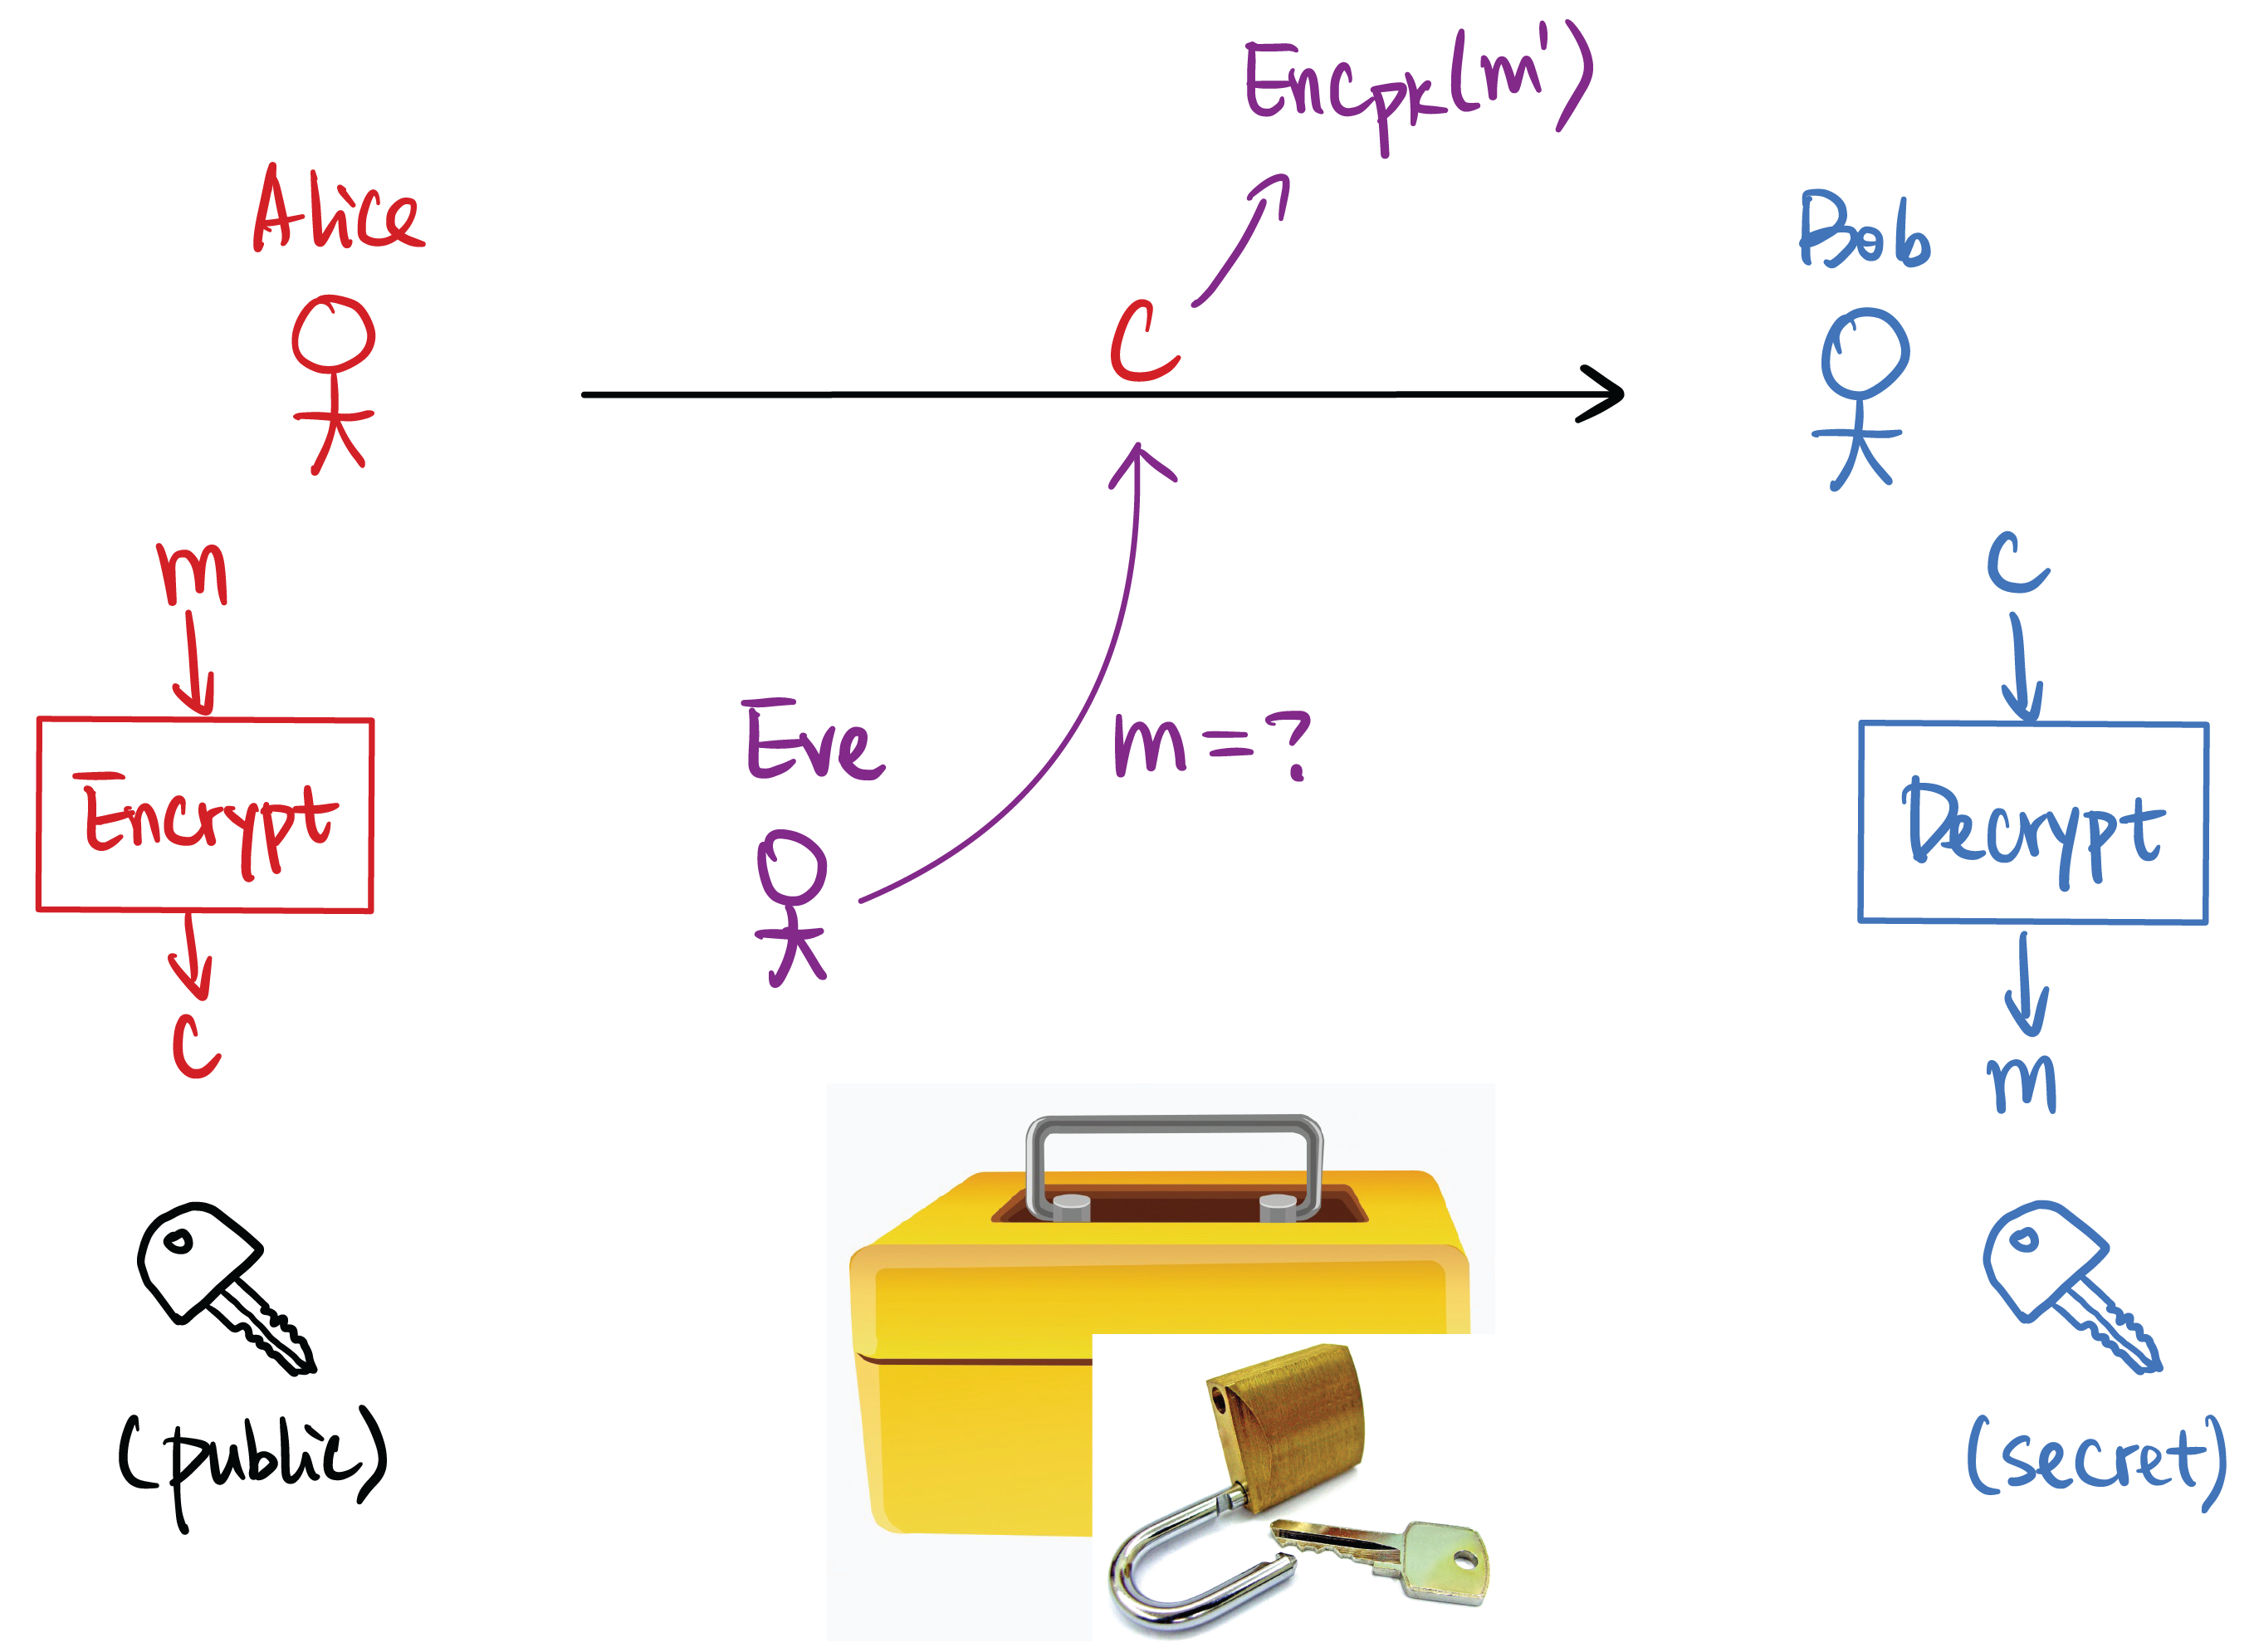
\includegraphics[width=0.9\textwidth]{images/2023-01-26/public_key.png}
    \end{center}

    This is seemingly magic! Bob could publish a public key on his homepage, anyone can encrypt using a public key but only Bob can decrypt. \emph{Stay tuned, we will see public-key encryption schemes next lecture!}
\end{definition}

\subsubsection{Message Integrity}
Alice wants to send a message to Bob again, but Eve is stronger! Eve can now tamper with the message.

\begin{center}
    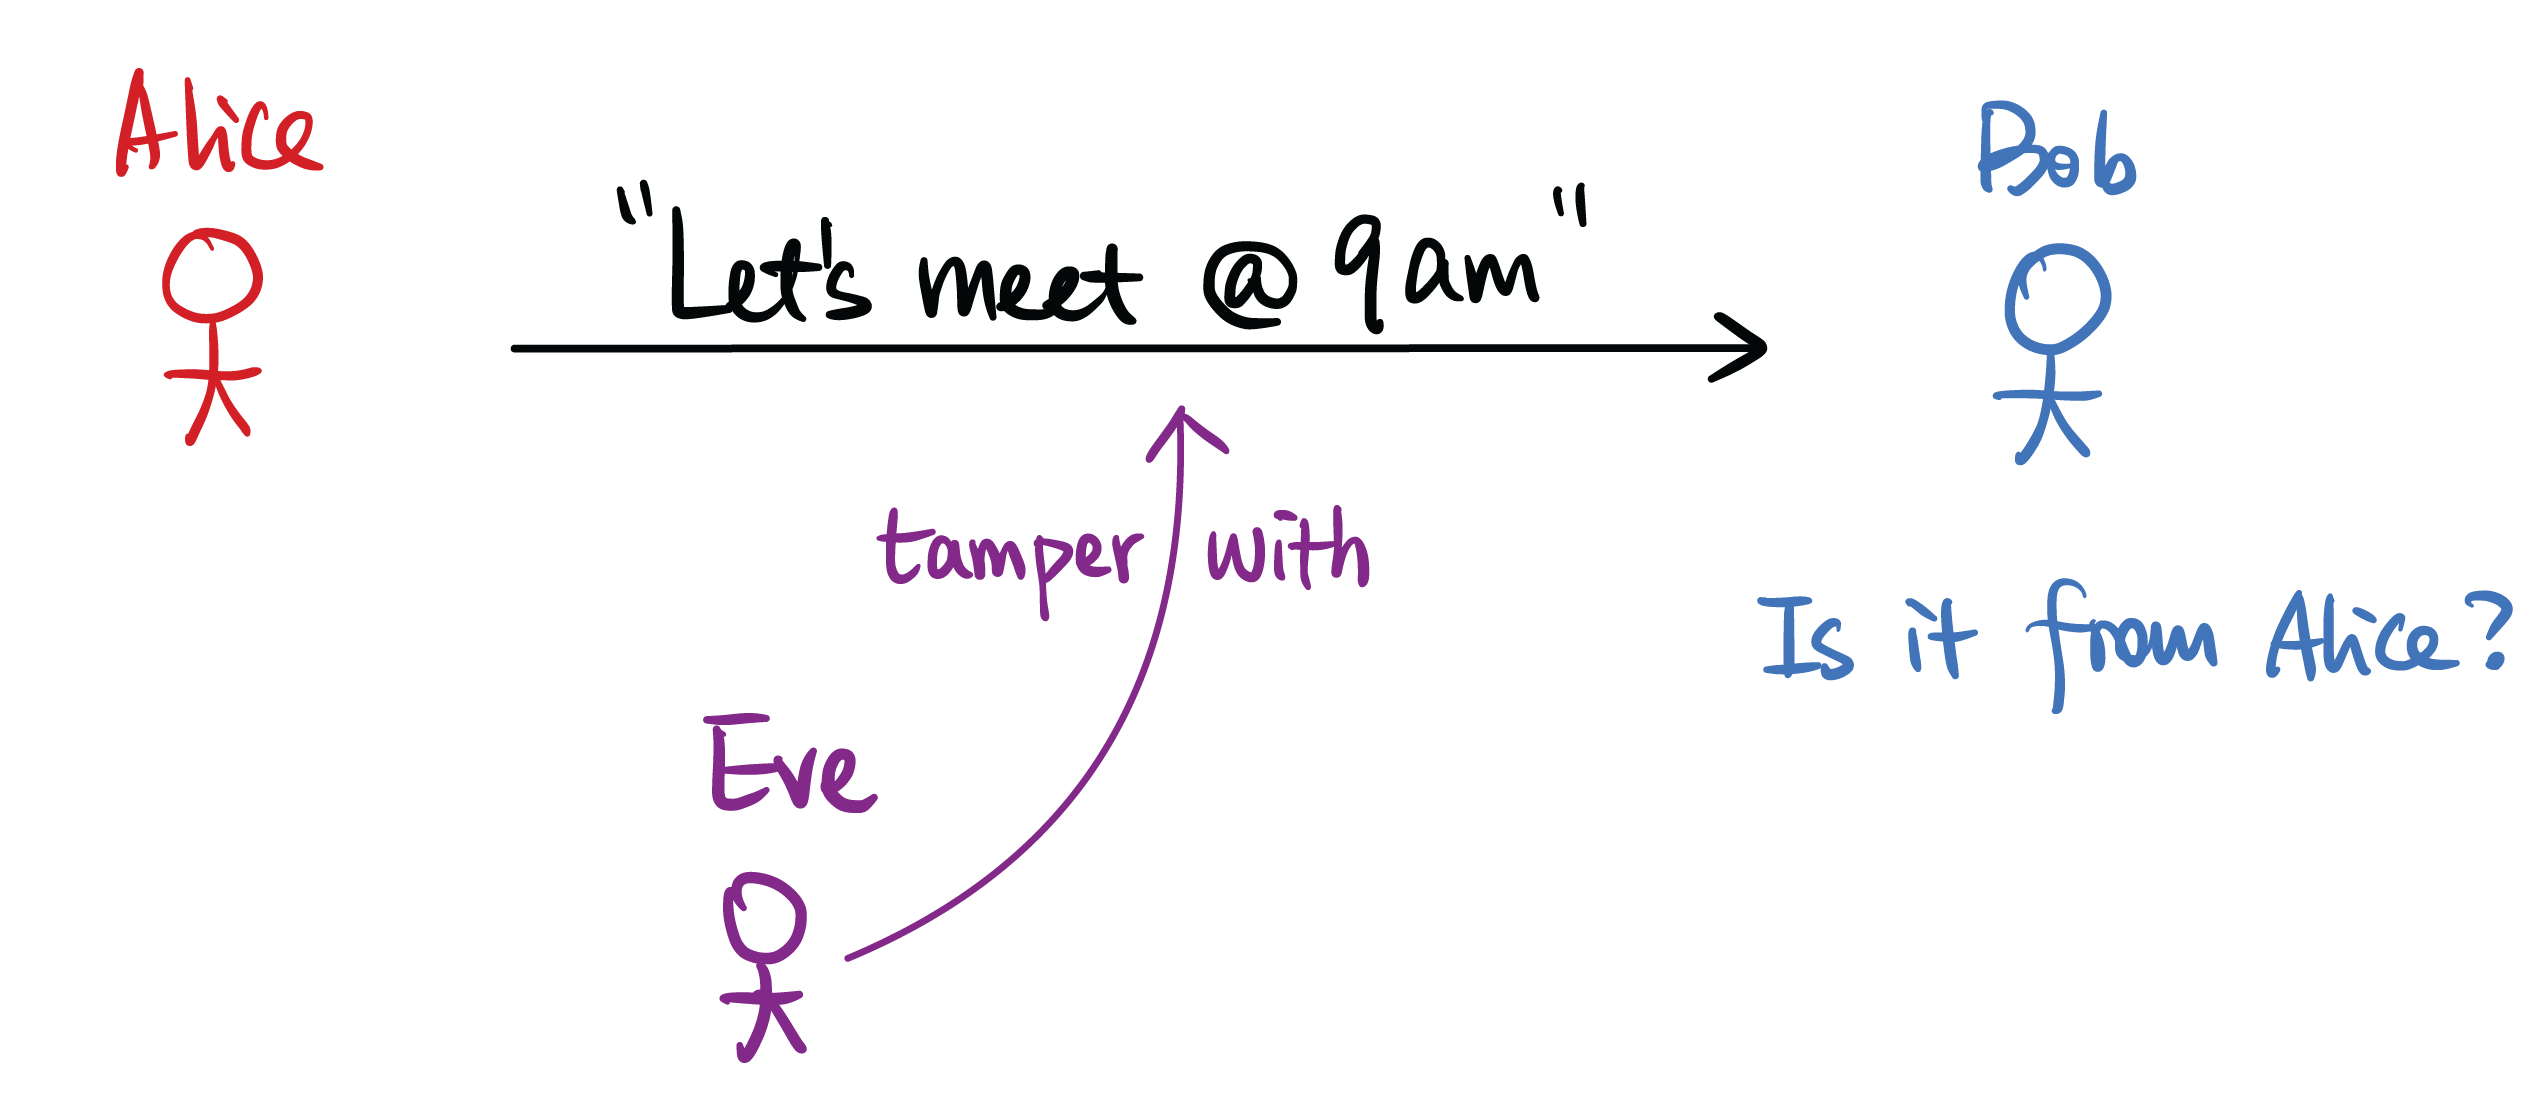
\includegraphics[width=0.9\textwidth]{images/2023-01-26/integrity.png}
\end{center}

Bob wants to ensure that the message \emph{actually} comes from Alice. Does our previous scheme (of encrypting messages) solve this problem? Nope!

Eve can change the ciphertext to something else, they could pretend to be Alice. In secret-key schemes, if Eve figures out the secret-key, they can forge messages from Alice. Even if Eve doesn't know the underlying message, they could still change it to some other ciphertext which might be correlated to the original ciphertext, \emph{without knowing the underlying message}. We'll see how Eve can meaningfully do this in some schemes. Alice could send a message ``Let's meet at $x$ AM'' and Eve could tamper this to say ``Let's meet at $x+1$ AM.''

This is sort of an orthogonal problem to message secrecy. For example, when Alice logs in to Google, Google needs to verify that Alice actually is who she claims to be.

\begin{center}
    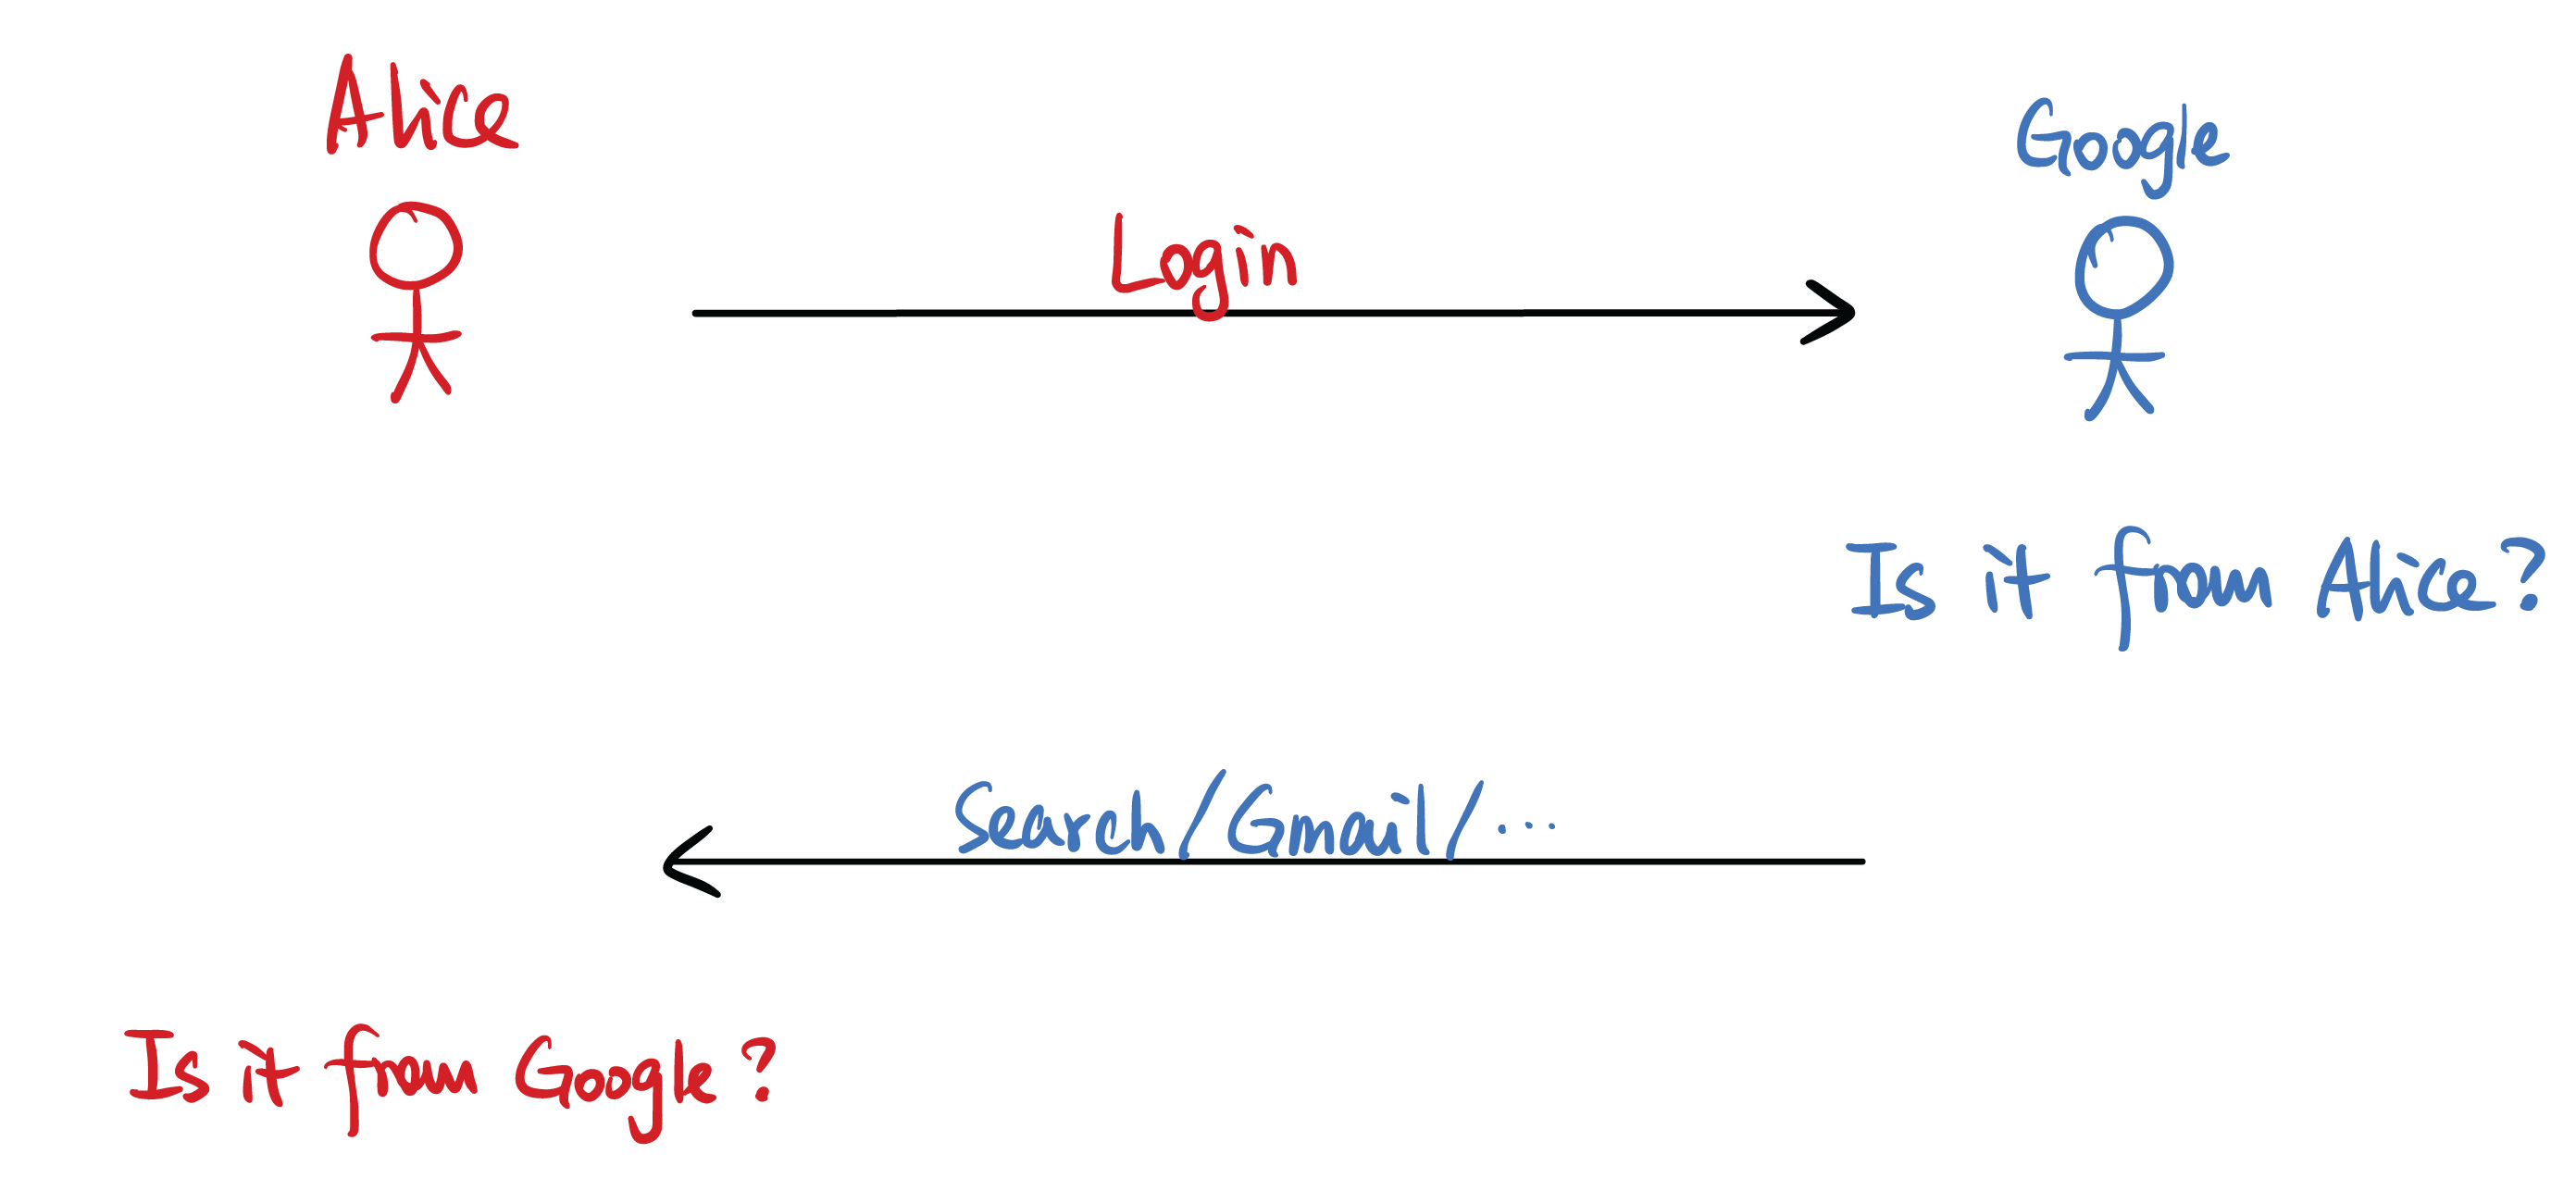
\includegraphics[width=0.9\textwidth]{images/2023-01-26/authentication.png}
\end{center}

This property that we want is called \ul{message integrity}.

\subsubsection{Signal and Auth}

The first two projects are Signal and Auth whose aim will be to cover \ul{secure messaging} and \ul{secure authentication}.

\emph{Projects Overview}
\begin{enumerate}
    \setcounter{enumi}{-1}
    \item Warm-up, you will implement some basic cryptographic schemes.
    \item Secure Communication: how to communicate in secret.
    \item Secure Authentication: how to authenticate yourself.
    \item Zero-Knowledge Proofs: we'll use ZKPs to implement a secure voting scheme.
    \item Secure Multiparty Computation: we'll implement a way to run any function securely between two parties.
    \item Fully Homomorphic Encryption: a form of post-quantum cryptography.
\end{enumerate}

We'll now introduce the latter three projects!

\subsection{Zero-Knowledge Proofs}
This is to prove something without \emph{revealing} any additional knowledge.

For example, Alice may want to
\begin{itemize}
    \item Prove she knows the difference in taste between Coke and Pepsi without revealing how
    \item Prove that you have a bug in your code without revealing the bug
    \item She has the secret key for this ciphertext without revealing the plaintext
\end{itemize}

How is this possible?
\begin{example*}
    Alice claims to be able to differentiate between Coca-Cola and Pepsi! She wants to prove this to Bob without revealing her secrets.

    Bob will randomly sample a bit $b\overset{\$}{\leftarrow}\{0, 1\}$, with $b=0$ being Coca-Cola and $b=1$ being Pepsi. Bob will let Alice taste this drink. Alice will give a guess $b'$ of what drink it is.

    \begin{center}
        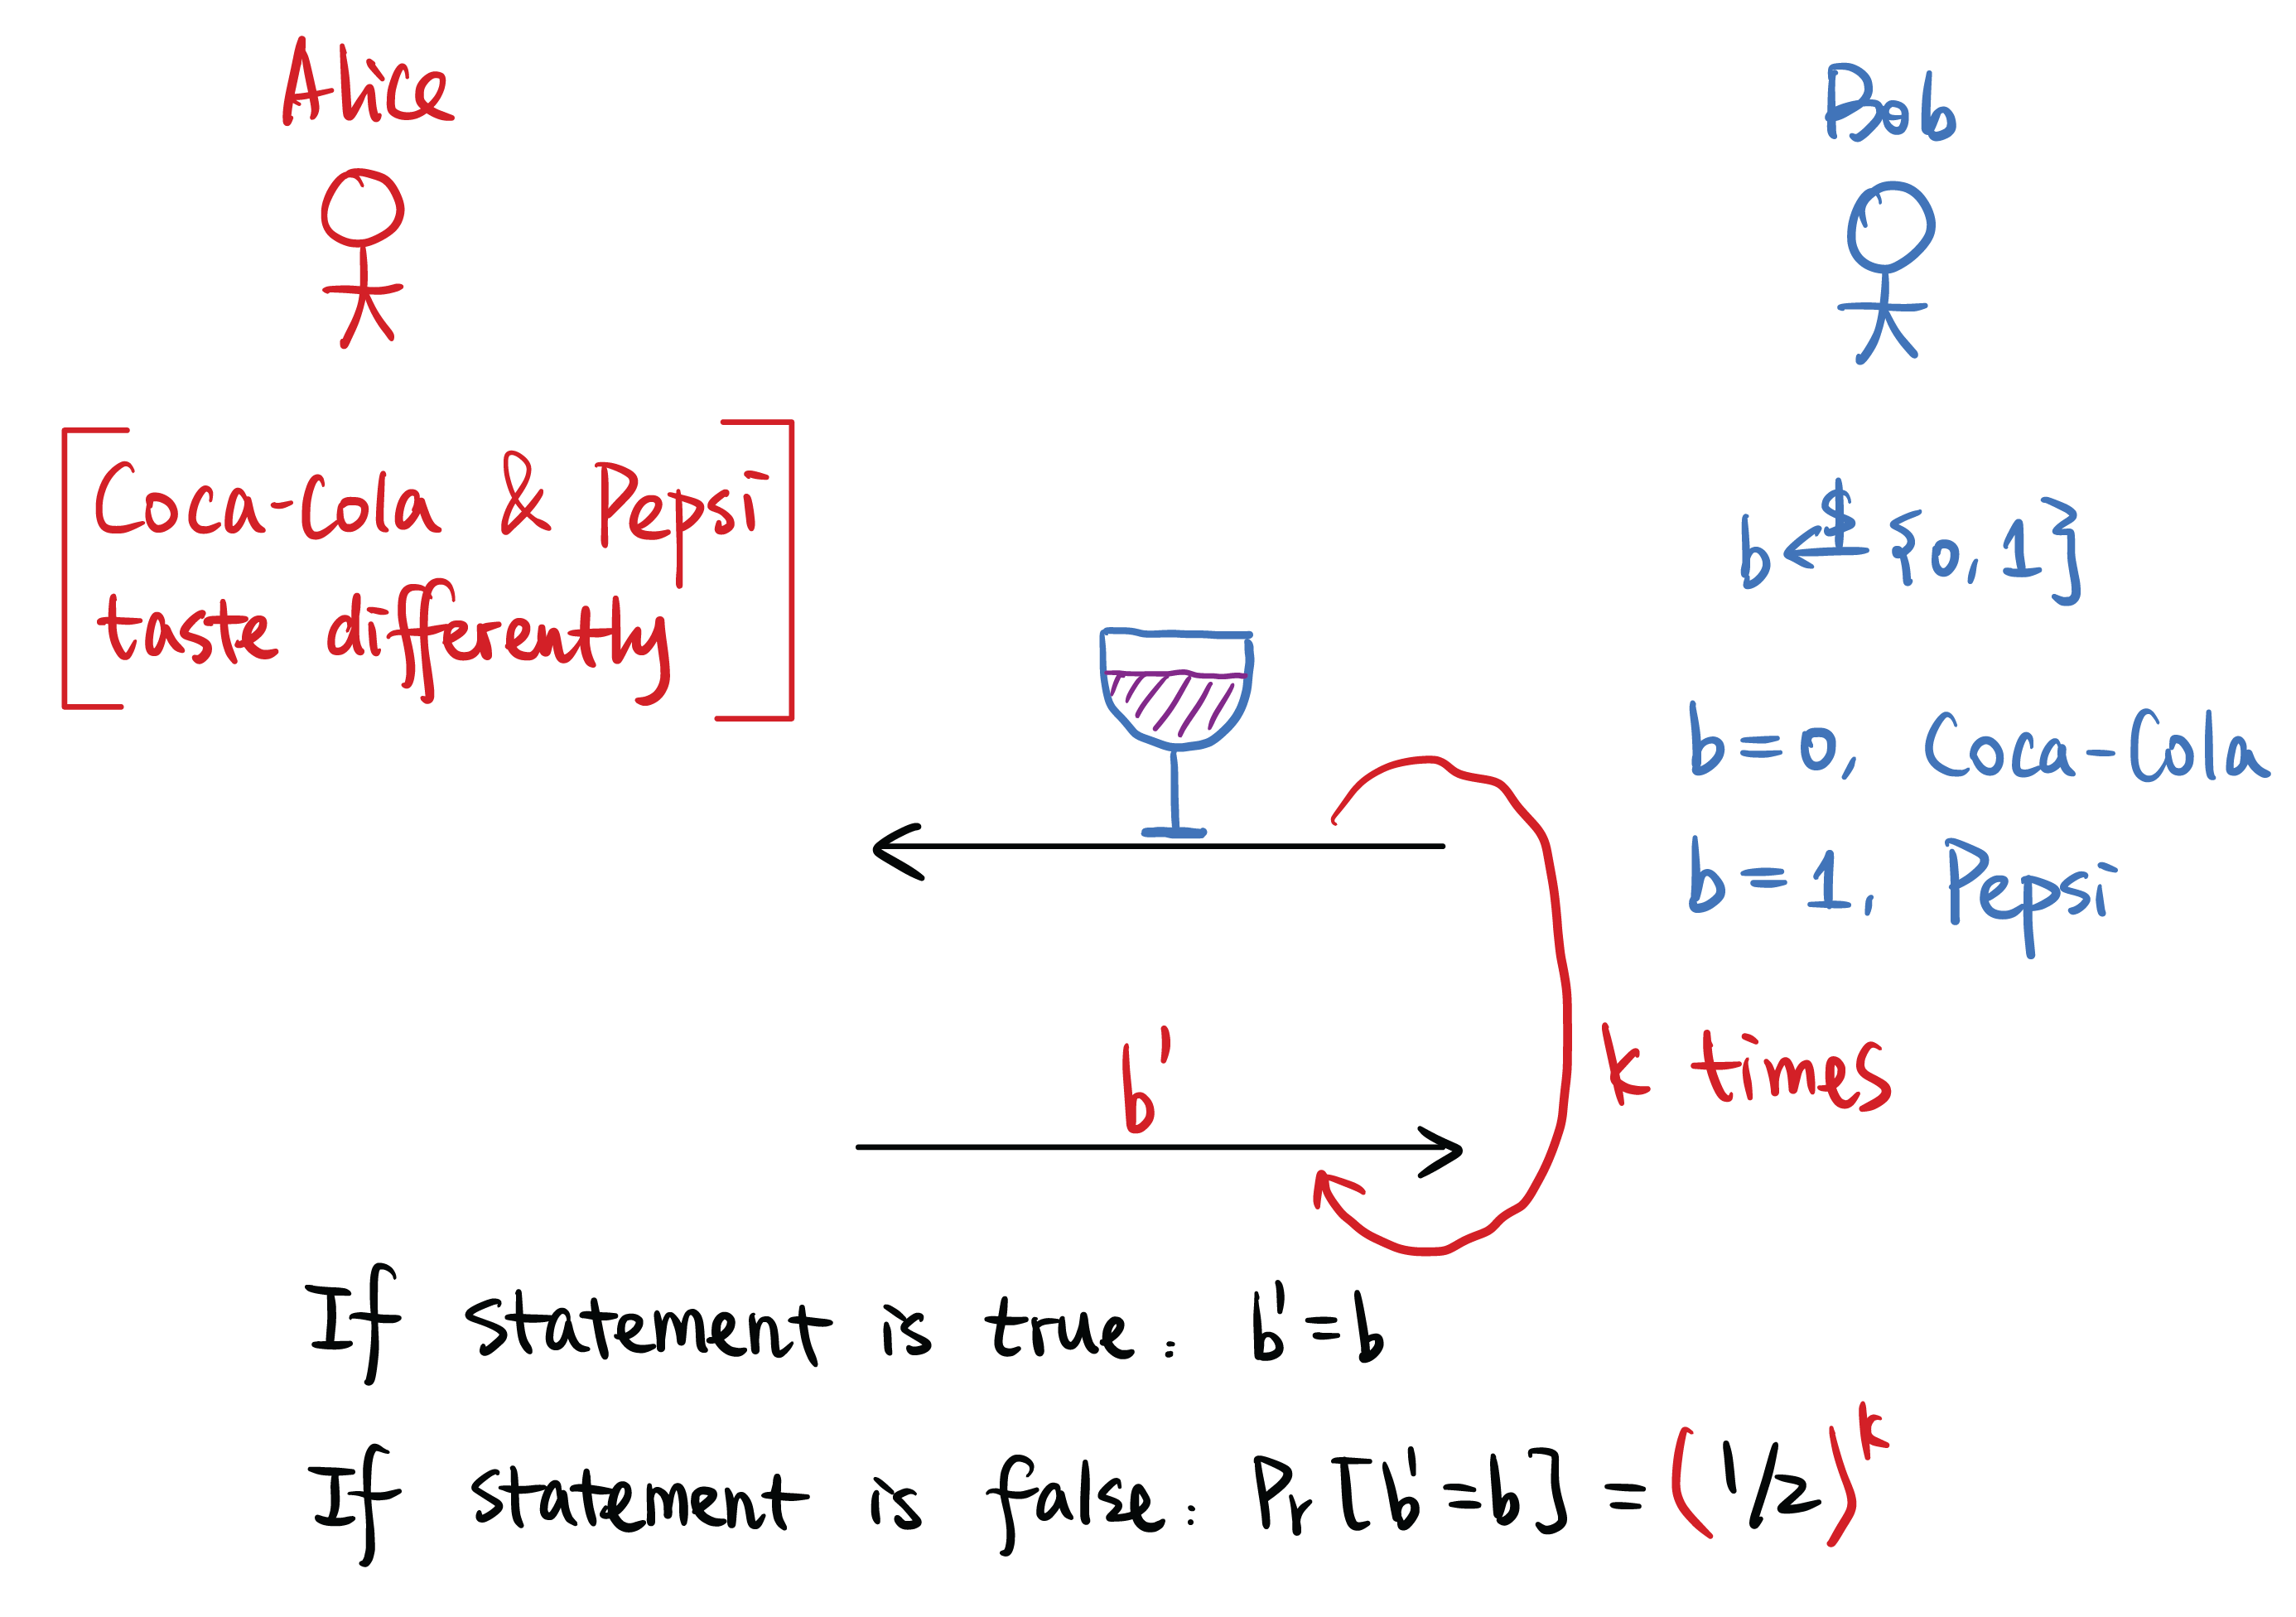
\includegraphics[width=0.9\textwidth]{images/2023-01-26/zk_cola.png}
    \end{center}

    If the statement is true, $\Pr[b' = b] = 1$ (Alice always gives the correct prediction).

    If the statement is false, $\Pr[b' = b] = \frac{1}{2}$ (Alice is guessing with $0.5$ probability).

    To enhance this, we can run this a total of $k$ times. If we run it enough times, Bob will be more and more confident in believing this. Alice getting this correct by chance has a $\frac{1}{2^k}$ probability.

    The key idea, however, is that Bob doesn't gain any knowledge of how Alice differentiates.

    \begin{remark*}
        This is a similar strategy in proving graph non-isomorphism.

        For people who have seen this before, generally speaking, any $\textsf{NP}$ language can be proved in zero-knowledge. Alice has the \emph{witness} to the membership in $\textsf{NP}$ language.
    \end{remark*}
\end{example*}

\subsection{Secure Multi-Party Computation}
\begin{center}
    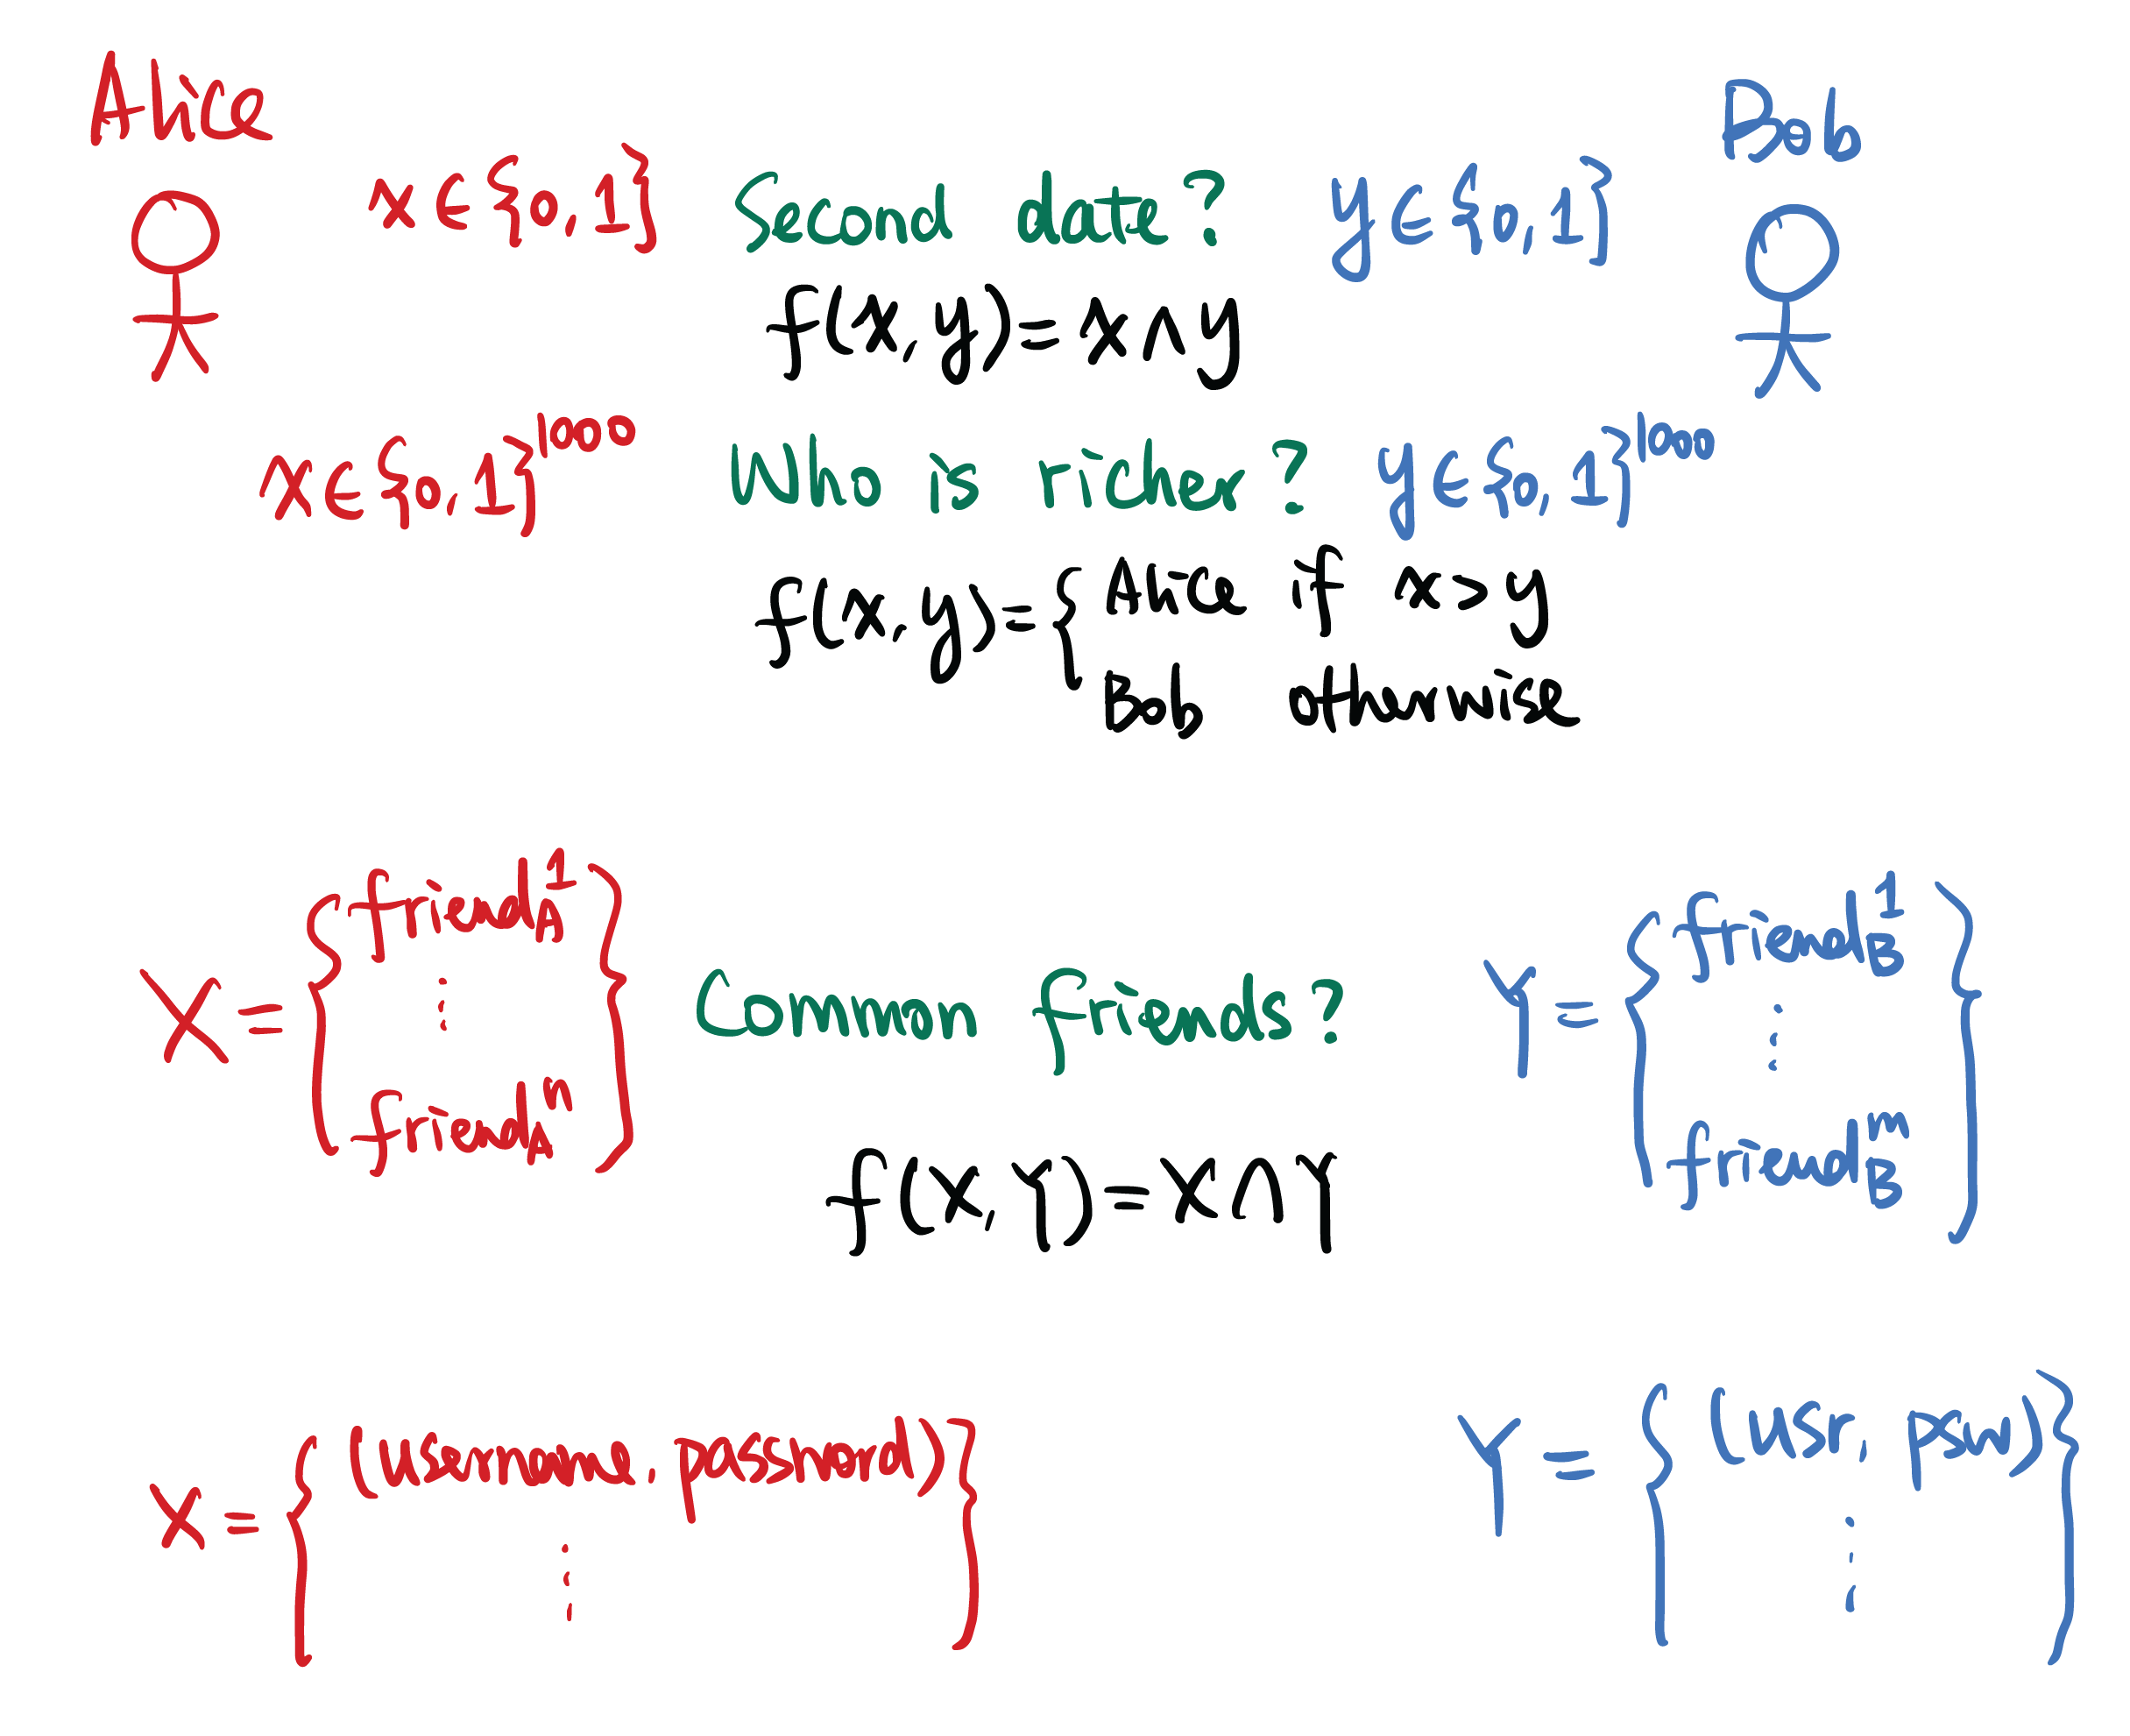
\includegraphics[width=0.9\textwidth]{images/2023-01-26/secure_mpc.png}
\end{center}

\begin{example*}[Secure \textsf{AND}]
    Alice and Bob go on a first date, and they want to figure out whether they want to go on a second date. They will only go on a second date if and only if both agree to a second date.

    How will they agree on this? They could tell each other, but this could be embarrassing. One way is for them to share with a third-party (this is what dating apps do!). However, there might not always be an appropriate third party (in healthcare examples, not everyone can be trusted with the data).

    In this case, Alice has a choice bit $x\in\{0, 1\}$ and Bob has a choice bit $y\in\{0, 1\}$. They are trying to jointly compute $f(x, y) = x\land y$.

    \begin{remark}
        Couldn't a party still figure out how the other party feels? For example, if Bob's bit was 1 and the joint result was 0, Bob can \emph{infer} that Alice's bit was 0.

        This is, in effect, the best we can do. The ideal guarantee is that each party only learns any information they can infer from the \emph{output} and their input. However, they should not learn anything more.
    \end{remark}
\end{example*}

What are we trying to achieve here? We want to jointly compute some function, where each party has private input, such that each party only learns the output. They should not learn anything about other partys' inputs.

\begin{example*}[Yao's Millionaires' Problem]
    Perhaps, Alice and Bob wants to figure out who is richer. The inputs are $x\in\{0, 1\}^{1000}$ and $y\in\{0, 1\}^{1000}$ (for simplification, let's say they can express their wealth in 1000 bits). The output is the person who has the max.
    \[f(x, y) = \begin{cases}
            \text{Alice} & \text{if }x > y  \\
            \text{Bob}   & \text{otherwise}
        \end{cases}\]
\end{example*}

\begin{example*}[Private Set Intersection]\label{ex:psi}
    Alice and Bob meet for the first time and want to determine which of their friends they share. However, they do not want to reveal who specifically are their friends.

    $X$ is a set of A's friends $X = \{\mathsf{friend}_A^1, \mathsf{friend}_A^2, \cdots, \mathsf{friend}_A^n\}$ and Bob also has a set $Y = \{\mathsf{friend}_B^1, \mathsf{friend}_B^2, \cdots, \mathsf{friend}_B^m\}$. They want to jointly compute \[f(X, Y) = X\cap Y.\]

    You might need to reveal the cardinality of these sets, but you could also pad them up to a maximum number of friends.

    This has a lot of applications in practice! In Google Chrome, your browser will notify you that your password has been leaked on the internet, without having access to your passwords in the clear. $X$ will be a set of \emph{your} passwords, and Google will have a set $Y$ of \emph{leaked} passwords. The \emph{intersection} of these sets are which passwords have been leaked over the internet, without revealing all passwords in the clear.
\end{example*}
\begin{ques*}
    Isn't the assumption that the size of input records is revealed weaker than using a trusted third-party?

    Yes, however in some cases (hospital health records), parties are legally obliged to keep data secure. We wish for security more than the secrecy of cardinality.
\end{ques*}

In the general case, Alice and Bob have some inputs $x$ and $y$ with bounded length, and they want to jointly compute some function $f$ on these inputs. This is \ul{Secure Two-Party Computation}. Furthermore, there could be multiple parties $x_1, \dots, x_n$ that jointly compute $f(x_1, \dots, x_n)$ that hides each input. This is \ul{Secure Multiparty Computation}.

We'll explore a toy example with the bit-\textsf{AND} from the dating example.

\begin{example*}[Private Dating]
    Alice and Bob have choice bits $x\in\{0, 1\}$ and $y\in\{0, 1\}$ respectively. There is a \emph{physical} round table with $5$ identical slots, one already filled in with a $1$ facing down.

    \begin{center}
        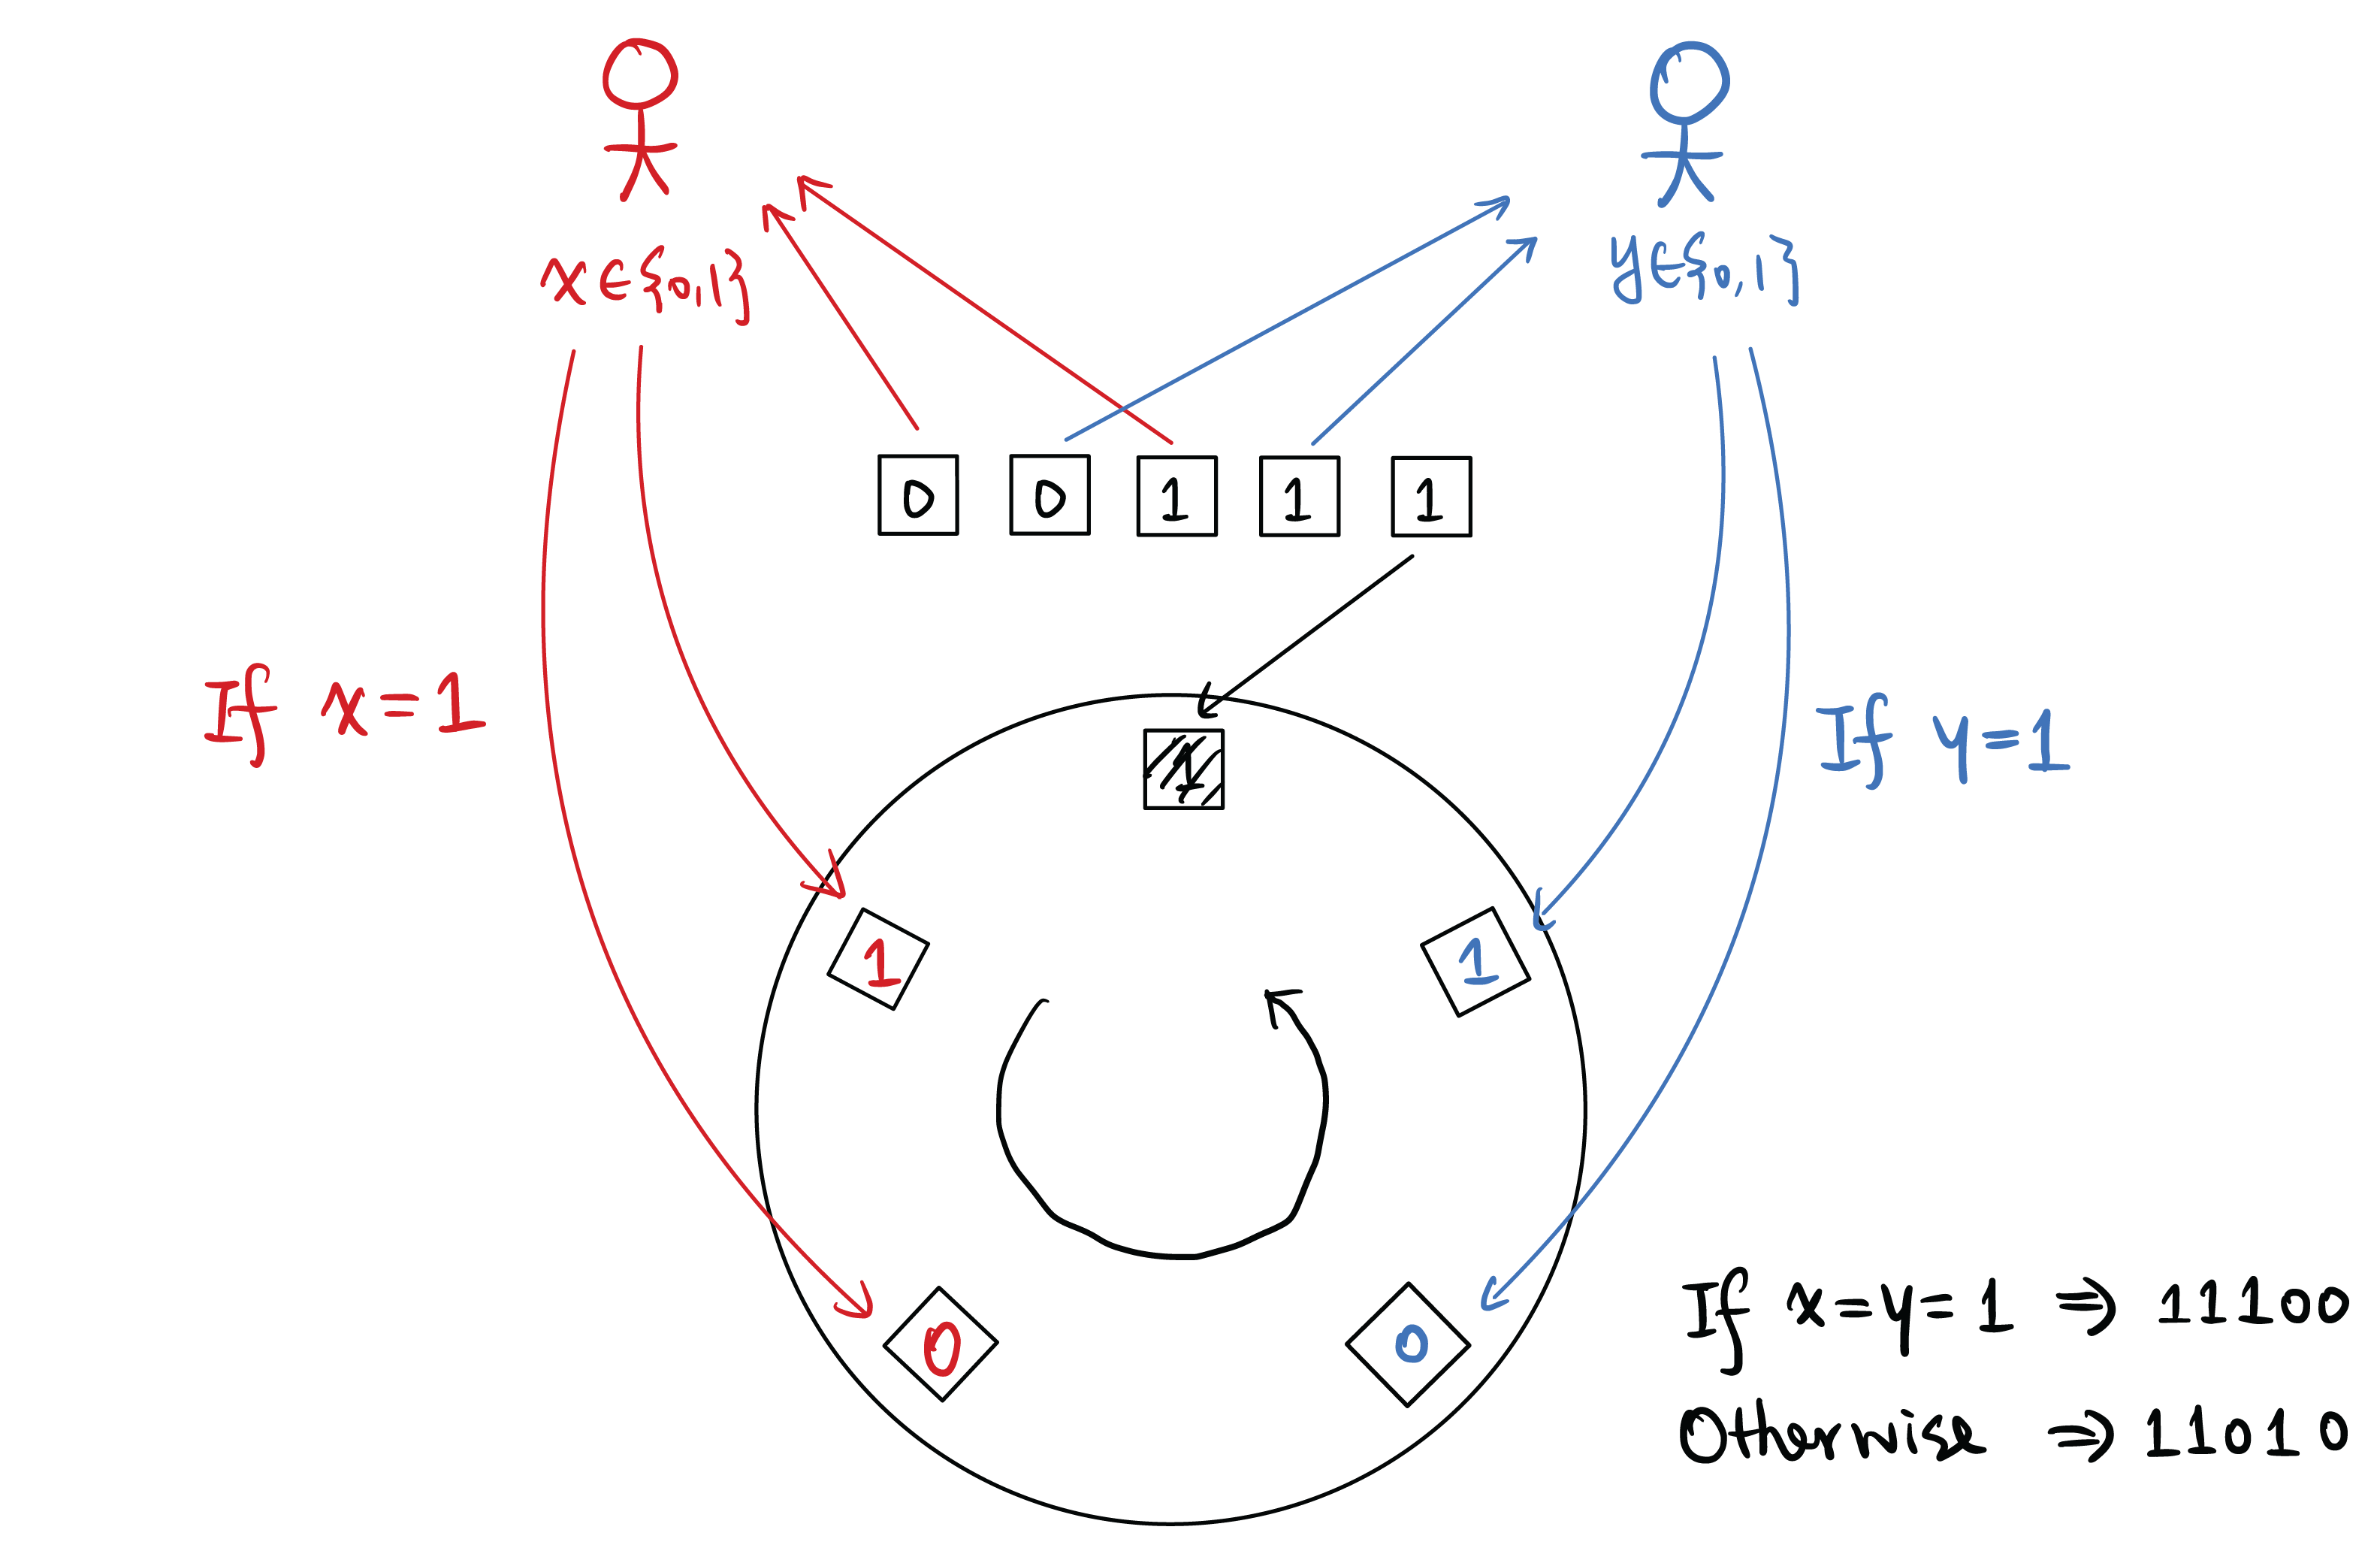
\includegraphics[width=0.9\textwidth]{images/2023-01-26/private_dating.png}
    \end{center}

    Alice and Bob each have identical $0, 1$ cards (each of the $0$ and $1$ cards are indistinguishable from cards of the same value). Alice places her cards on the 2 slots in some order, and Bob does the same.

    They then spin the table around and reveal all the cards, learning $x\land y$.

    If $x = 1$, Alice places it as $1$ on top of $0$, and if $y = 1$, Bob places it as $1$ on top of $0$ as well. Otherwise, they flip them. If $x = y = 1$, then the $0$'s will be adjacent. If $x \neq y$, the order will be $1,1,0,1,0$ (the $0$'s are not adjacent), regardless of which of Alice or Bob produced $x = 0$ (or both!).
\end{example*}

\emph{This is a toy example! It doesn't use cryptography at all! Two parties have to sit in front of a table. This is called card-based cryptography. We will be using more secure primitives.}

\subsection{Fully Homomorphic Encryption}
We'll come back to the secure messaging example.

Alice wants to send Bob a message. She encrypts it somehow and sends a ciphertext $c_1 = \mathsf{Enc}(m_1)$. A nice feature for some encryption schemes is for Eve to do some computation homomorphically on the ciphertexts. Eve might possibly want to add ciphertexts (that leads to plaintext adding)
\[c_1 = \mathsf{Enc}(m_1),\ c_2 = \mathsf{Enc}(m_2)\Rightarrow c' = \mathsf{Enc}(m_1 + m_2)\]
or perhaps $c'' = \mathsf{Enc}(m_1\cdot m_2)$, or compute arbitrary functions. \emph{Sometimes}, this is simply adding $c_1 + c_2$, but usually not.

\begin{center}
    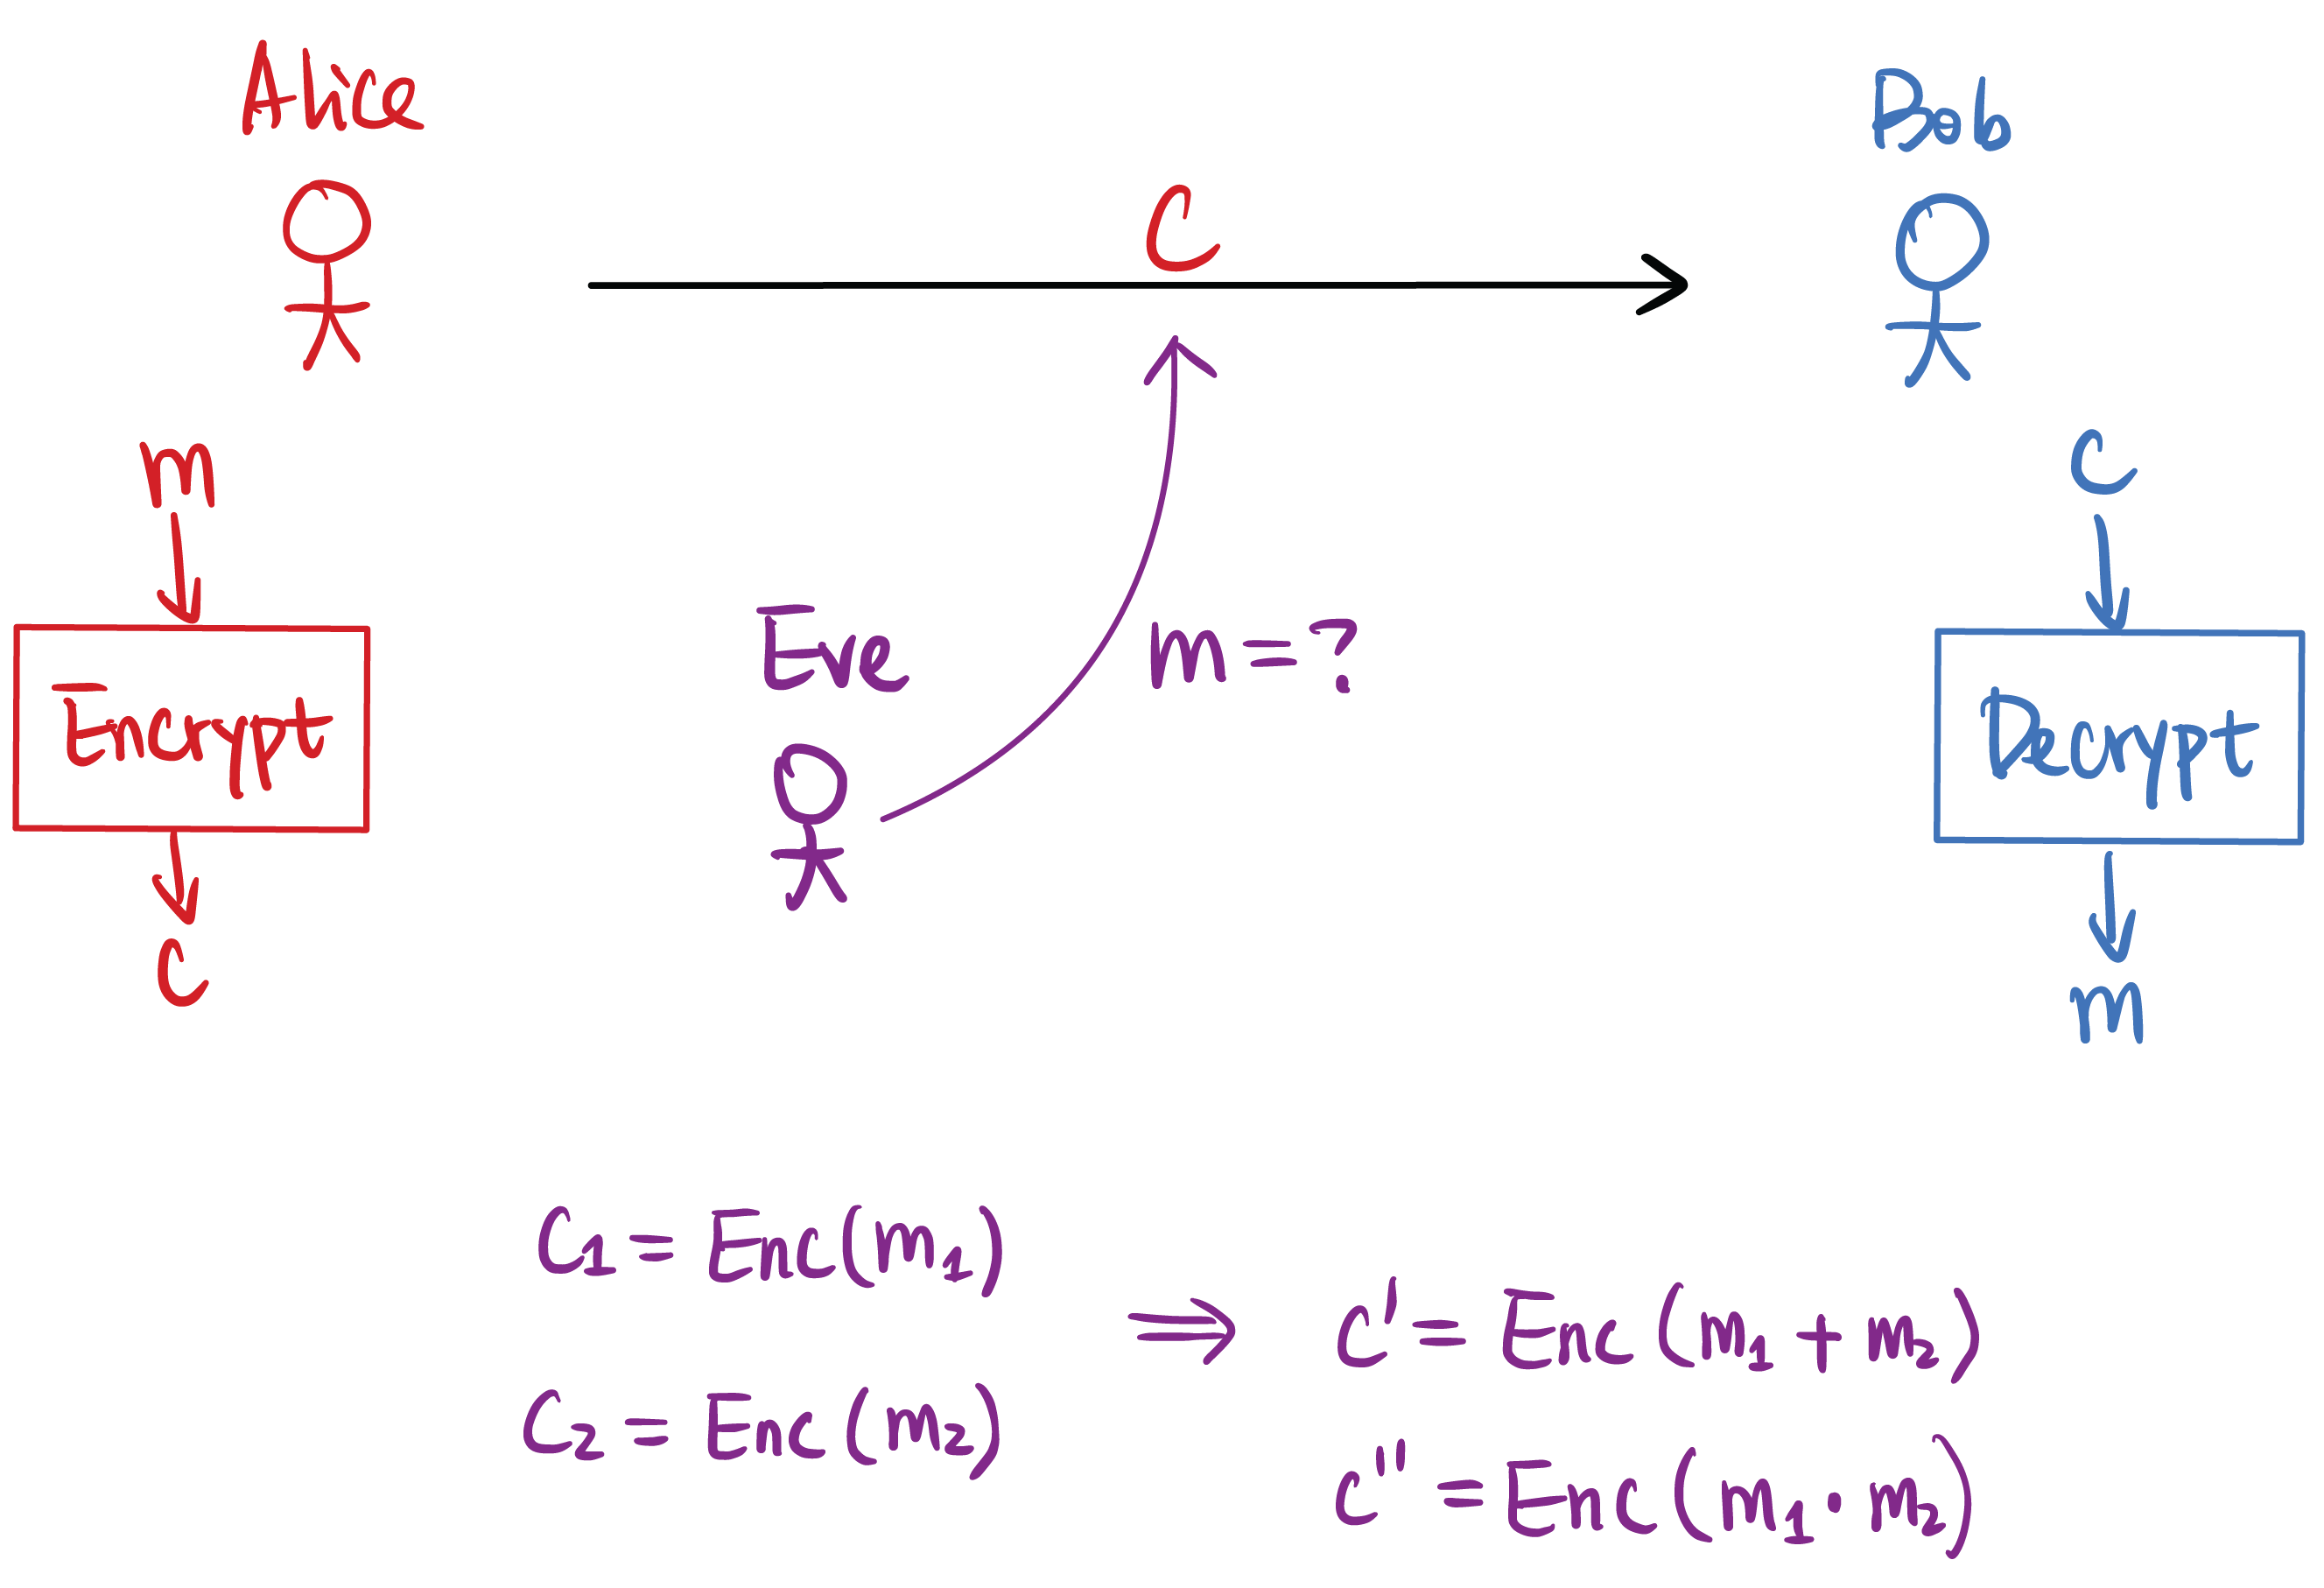
\includegraphics[width=0.9\textwidth]{images/2023-01-26/homomorphic_encryption.png}
\end{center}

We want to hopefully compute any function in polynomial time!

\begin{example*}[Outsourced Computation]
    Alice has some messages but doesn't have enough compute. There is a server that has \emph{a lot} of compute!

    \begin{center}
        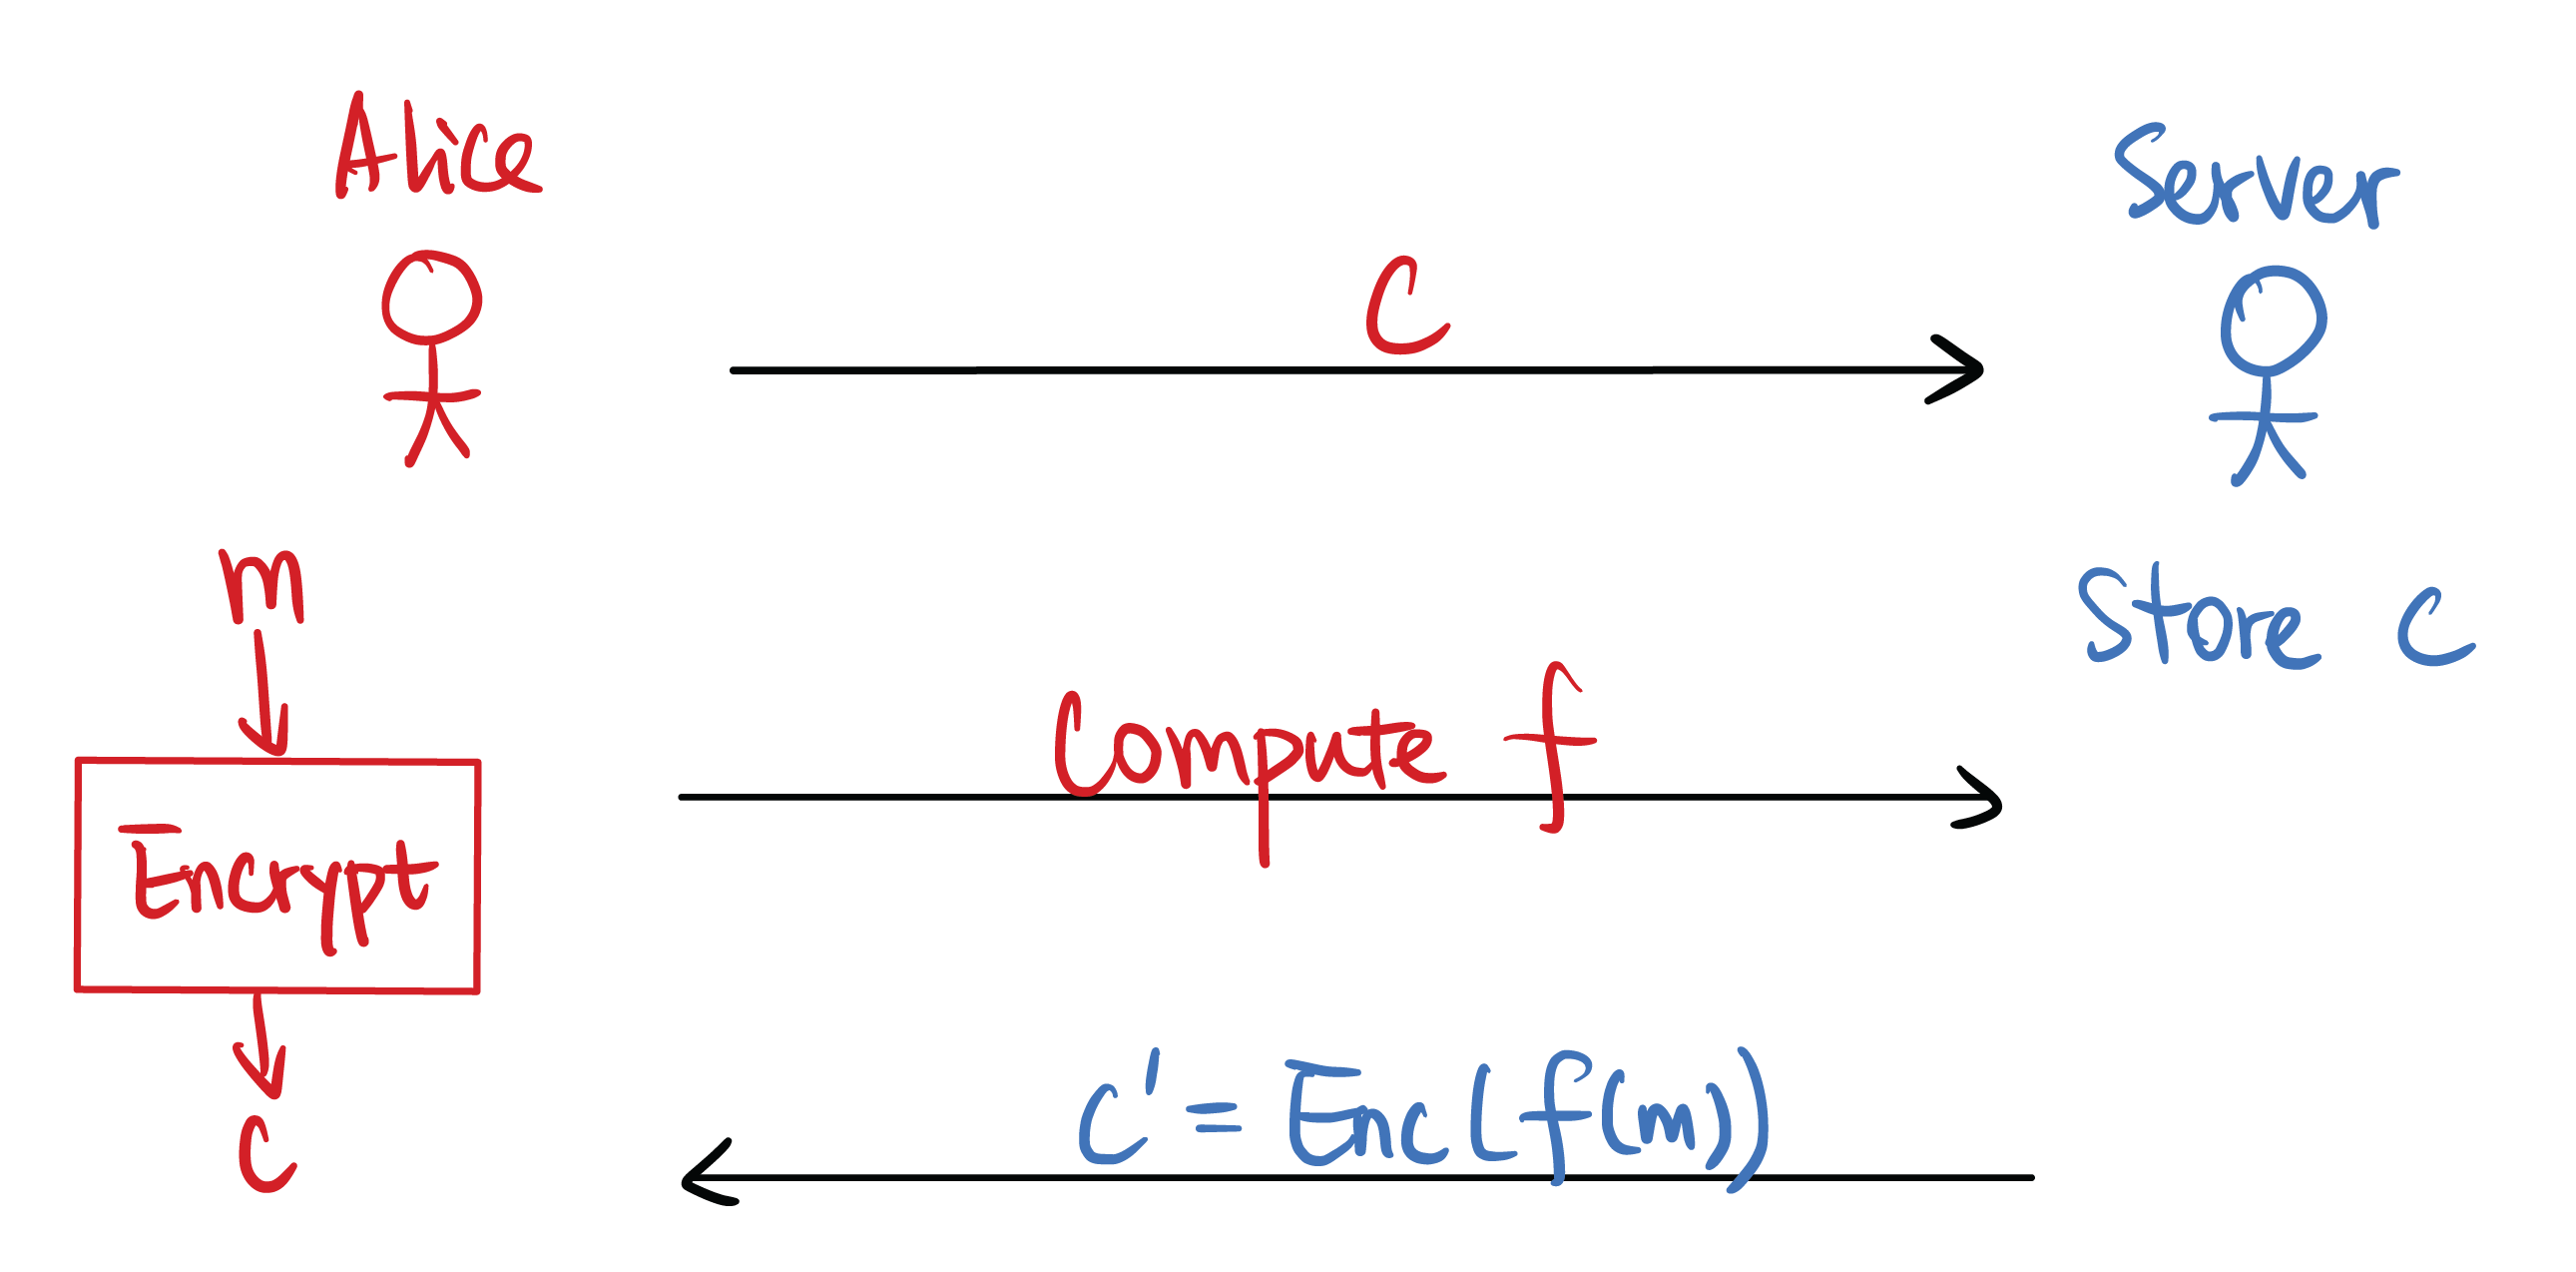
\includegraphics[width=0.9\textwidth]{images/2023-01-26/outsourced_computation.png}
    \end{center}

    Alice encrypts her data and stores it in the server. At some point, Alice might want to compute a function on the encrypted data on the server, without the server revealing the original data.

    This is an example of how fully homomorphic encryption can be useful.
\end{example*}

\begin{remark*}
    This problem was not solved until 2009 (when Peihan started her undergrad). Theoretically, it doesn't even seem that possible! Being able to compute functions on ciphertexts that correspond to functions on plaintexts.
\end{remark*}

To construct fully-homomorphic encryption, we'll be using lattice-based cryptography which is a post-quantum secure!

\subsection{Further Topics}
We might cover some other topics:
\begin{itemize}
    \item Differential Privacy
    \item Crypto applications in machine learning
    \item Crypto techniques used in the blockchain\footnote{One important techniques is Zero-Knowledge proofs, for example.}
\end{itemize}
\emph{What else would you like to learn? What else do you want to understand?} Do go through the semester with these in mind! \emph{How do I log into Google? How do I send messages to friends?}

Feel free to let us know on Ed!

\subsection{Q \& A}

\begin{itemize}
    \item \emph{What is the difference between CSCI 1515 and CSCI 1510 or MATH 1580?}
    
    CSCI 1510 is essentially ``theoretical cryptography.'' It covers formal definitions and constructions and proofs. There is no coding, just proofs.

    MATH 1580 considers crypto from the mathematical perspective. They try to understand some of the computational assumptions we assume from a mathematical standpoint. I.e. why is factoring hard to compute, and what is the best algorithm to compute it? In CS, we simply assume factoring is hard. MATH 1580 is more similar to number theory and group theory.

    \item \emph{If you've taken MATH 1580 and CSCI 1515, would you still recommend taking CSCI 1510?}
    
    There are still more things to learn from CSCI 1510. There is still more theory and it is a much more challenging course from the theoretical perspective. There are more rigorous proofs and reductions in CSCI 1510 that we do not cover in CSCI 1515.

    \item \emph{Why C++}

    Existing crypto libraries are mostly in C++ and most students have seen C/C++ in either cs33 or cs300. We did, however, consider implementing everything in Rust!
\end{itemize}
